\newcommand{\econtexRoot}{.}
% The \commands below are required to allow sharing of the same base code via Github between TeXLive on a local machine and ShareLaTeX.  This is an ugly solution to the requirement that custom LaTeX packages be accessible, and that ShareLaTeX seems to ignore symbolic links (even if they are relative links to valid locations)
\providecommand{\econtex}{\econtexRoot/texmf-local/tex/latex/econtex}
\providecommand{\econtexSetup}{\econtexRoot/texmf-local/tex/latex/econtexSetup}
\providecommand{\econtexShortcuts}{\econtexRoot/texmf-local/tex/latex/econtexShortcuts}
\providecommand{\econtexBibMake}{\econtexRoot/texmf-local/tex/latex/econtexBibMake}
\providecommand{\econtexBibStyle}{\econtexRoot/texmf-local/bibtex/bst/econtex}
\providecommand{\notes}{\econtexRoot/texmf-local/tex/latex/handout}
\providecommand{\handoutSetup}{\econtexRoot/texmf-local/tex/latex/handoutSetup}
\providecommand{\handoutShortcuts}{\econtexRoot/texmf-local/tex/latex/handoutShortcuts}
\providecommand{\handoutBibMake}{\econtexRoot/texmf-local/tex/latex/handoutBibMake}
\providecommand{\handoutBibStyle}{\econtexRoot/texmf-local/bibtex/bst/handout}

  
\documentclass[titlepage]{\econtex}\newcommand{\texname}{cAndCwithStickyE}
\usepackage{\econtexSetup}\usepackage{\econtexShortcuts}
\usepackage[nolists,nomarkers,tablesonly]{endfloat}
\usepackage{titlesec}
\setcounter{secnumdepth}{4}

\provideboolean{ifWeb}
\setboolean{ifWeb}{false}
\opt{Web}{\setboolean{ifWeb}{true}}

\ifthenelse{\boolean{ifWeb}}{\usepackage{grfext}
\PrependGraphicsExtensions*{.svg,.jpg,.JPG,.png,.PNG,.pdf,.PDF}
}{}


\titleformat{\paragraph}
{\sffamily\mdseries\normalsize}{\theparagraph}{1em}{}
\titlespacing*{\paragraph}
{0pt}{3.25ex plus 1ex minus .2ex}{1.5ex plus .2ex}

\hypersetup{pdfauthor={Christopher Carroll <ccarroll@jhu.edu>, Edmund Crawley <ecrawle2@jhu.edu>, Jiri Slacalek <jiri.slacalek@ecb.europa.eu>, Kiichi Tokuoka <kiichi.tokuoka@mof.go.jp>, Matthew N White <mnwecon@udel.edu>},
            pdftitle={Sticky Expectations and Consumption Dynamics},
            pdfsubject={Sticky Expectations and Consumption Dynamics},
            pdfkeywords={Sticky Expectations, Consumption Dynamics, Habit Formation, Inattention; JEL: E21, F41},
            pdfproducer = {LaTeX with hyperref and thumbpdf},
            pdfcreator = {pdflatex}
            }

\newlength\TableWidth

\provideboolean{StandAlone}
\setboolean{StandAlone}{false}
\write18{\TabsDir/StandAloneOff.command} % Tell input files that they are being pulled in from the master (and are not standalone documents)

%rm%\provideboolean{PrintVersion}
%rm%\setboolean{PrintVersion}{false}
%rm%\setboolean{PrintVersion}{true}

\begin{document}\bibliographystyle{\econtexBibStyle}

\input Switches.tex

\begin{verbatimwrite}{\jobname.title}
Sticky Expectations and Consumption Dynamics
\end{verbatimwrite}

\hfill{\tiny \jobname}

\title{Sticky Expectations and \\ Consumption Dynamics}

\ifthenelse{\boolean{ifWeb}}{
\author{
  Christopher D. Carroll\authNum
  \and
  Edmund Crawley\authNum 
  \and
  Jiri Slacalek\authNum  
  \and
  Kiichi Tokuoka\authNum 
  \and
  Matthew N. White\authNum
}
}{
\author{
  Christopher D. Carroll\authNum \\ {\small JHU}
  \and
  Edmund Crawley\authNum   \\ {\small JHU}
  \and
  Jiri Slacalek\authNum    \\ {\small ECB}
  \and
  Kiichi Tokuoka\authNum   \\ {\small MoF Japan}
  \and
  Matthew N. White\authNum \\ {\small U of Delaware}
}
} % End ifWeb

\keywords{Consumption, Sticky Expectations, Habits, Inattention, Imperfect Information}
\jelclass{D83, D84, E21, E32}
% \aspublished{Final version as published in [].}

\date{February 20, 2018}
\maketitle

\begin{abstract}
  \opt{JournalFormatting}{\doublespacing}
  \begin{verbatimwrite}{./.abstract.metadata} 
    Macroeconomic models often invoke consumption ``habits'' to explain the substantial persistence of aggregate consumption growth. But a large literature has found no evidence of habits in the (vastly larger) microeconomic datasets that measure the behavior of individual households.  We show that the apparent conflict can be explained by a model in which consumers have accurate knowledge of their personal circumstances but `sticky expectations' about the macroeconomy. In our model, the persistence of aggregate consumption growth reflects consumers' imperfect attention to aggregate shocks. Our proposed degree of (macro) inattention has negligible utility costs, because aggregate shocks constitute only a tiny proportion of the uncertainty that consumers face.  In contrast with models in the existing literature, our model is consistent with {\it both} micro {\it and} macro stylized facts about consumption dynamics.
  \end{verbatimwrite}{./.abstract.metadata} 
  \input{./.abstract.metadata}
\end{abstract}

\ifthenelse{\boolean{ifWeb}}{}{\begin{small}}
\parbox{\textwidth}{
  \begin{center}
\begin{tabbing}
\texttt{Archive:~} \= \= \url{http://econ.jhu.edu/people/ccarroll/papers/cAndCwithStickyE.pdf} \kill \\  % This line establishes the locations of the tabs, but is not printed because of the \kill directive
\texttt{~~~~PDF:~} \> \> \url{http://econ.jhu.edu/people/ccarroll/papers/cAndCwithStickyE.pdf} \\
\texttt{~~~~Web:~} \> \> \url{http://econ.jhu.edu/people/ccarroll/papers/cAndCwithStickyE/} \\
\texttt{Archive:~} \> \> \url{http://econ.jhu.edu/people/ccarroll/papers/cAndCwithStickyE.zip} \\
\texttt{~Slides:~} \> \> Versions to \href{http://econ.jhu.edu/people/ccarroll/papers/cAndCwithStickyE-Slides.pdf}{View} or \href{http://econ.jhu.edu/people/ccarroll/papers/cAndCwithStickyE-Slides-Print.pdf}{Print} \\
\texttt{Toolkit:~} \> \> \url{http://github.com/Econ-ARK/HARK} \\
%\texttt{~~~~~~~~~} \> \> {\it (Contains data and estimation software producing paper's results)}
\end{tabbing}
\end{center}
}
\ifthenelse{\boolean{ifWeb}}{}{\end{small}}

\begin{authorsinfo}
  \name{Carroll: Department of Economics, Johns Hopkins University, \url{http://econ.jhu.edu/people/ccarroll/}, \href{mailto:ccarroll@jhu.edu}{\texttt{ccarroll@jhu.edu}}}
\name{Crawley: Department of Economics, Johns Hopkins University, \href{mailto:ecrawle2@jhu.edu}{\texttt{ecrawle2@jhu.edu}}}
\name{Slacalek: DG Research, European Central Bank, \url{http://www.slacalek.com/}, \href{mailto:jiri.slacalek@ecb.europa.eu}{\texttt{jiri.slacalek@ecb.europa.eu}}}
\name{Tokuoka: Ministry of Finance, Japan, \href{mailto:kiichi.tokuoka@mof.go.jp}{\texttt{kiichi.tokuoka@mof.go.jp}}}
\name{White: Department of Economics, University of Delaware,  \href{mailto:mnwecon@udel.edu}{\texttt{mnwecon@udel.edu}}}
\end{authorsinfo}
\thanks{The computational results in this paper were constructed using tools in the \href{http://github.com/Econ-ARK/HARK}{Econ-ARK/HARK} toolkit.  The toolkit can be cited by its digital object identifier, \href{https://doi.org/10.5281/zenodo.1001068}{10.5281/zenodo.1001068}, in the references as \cite{matthew_n_white_2017_1001068}.  Thanks to Robert King, Bartosz Ma\'ckowiak, Kathrin Schlafmann, Gianluca Violante and seminar participants in the NBER Summer Institute, the Copenhagen Conference on Heterogeneity, the McMaster University, the University of Michigan, and the University of Delaware for constructive and insightful comments which substantially improved this paper. The views presented in this paper are those of the authors, and should not be attributed to the European Central Bank or to the Japanese Ministry of Finance.}

\titlepagefinish
\setcounter{page}{1}

\pagebreak

%rm%\provideboolean{SlidesInText}
%rm%\setboolean{SlidesInText}{true}

\section{Introduction}

Starting with \cite{cdSmooth}, the macroeconomics, finance, and international economics literatures have established that aggregate consumption exhibits `excess smoothness' compared with the benchmark \cite{hallRandomWalk} random walk model of consumption.\footnote{In finance, early references are \cite{abel:aerhabits} and \cite{constantinidesHabits}; in international economics, \cite{gru04}.}  Over the past two decades many papers in these fields have responded to this problem by incorporating `habit formation' in the utility function of a representative agent.

This literature typically measures excess smoothness with a parameter conventionally labeled as the `habit formation coefficient' (which we denote as $\chi$). A recent comprehensive meta-analysis of 597 published estimates (\cite{hrsHabit}) reports that studies based on macro data find that $\chi=0.6$ on average; see Figure~\ref{microMacroMetaHistogram}.\footnote{For examples of such studies, see results and references in \cite{fuhrer:habits} or \cite{cee:habits}.}

\begin{figure}
\caption{Distribution of Estimates of Habit Persistence in Macro and Micro Studies}
\label{microMacroMetaHistogram}
\ifthenelse{\boolean{ifWeb}}{
  \begin{minipage}{\textwidth}
      \centerline{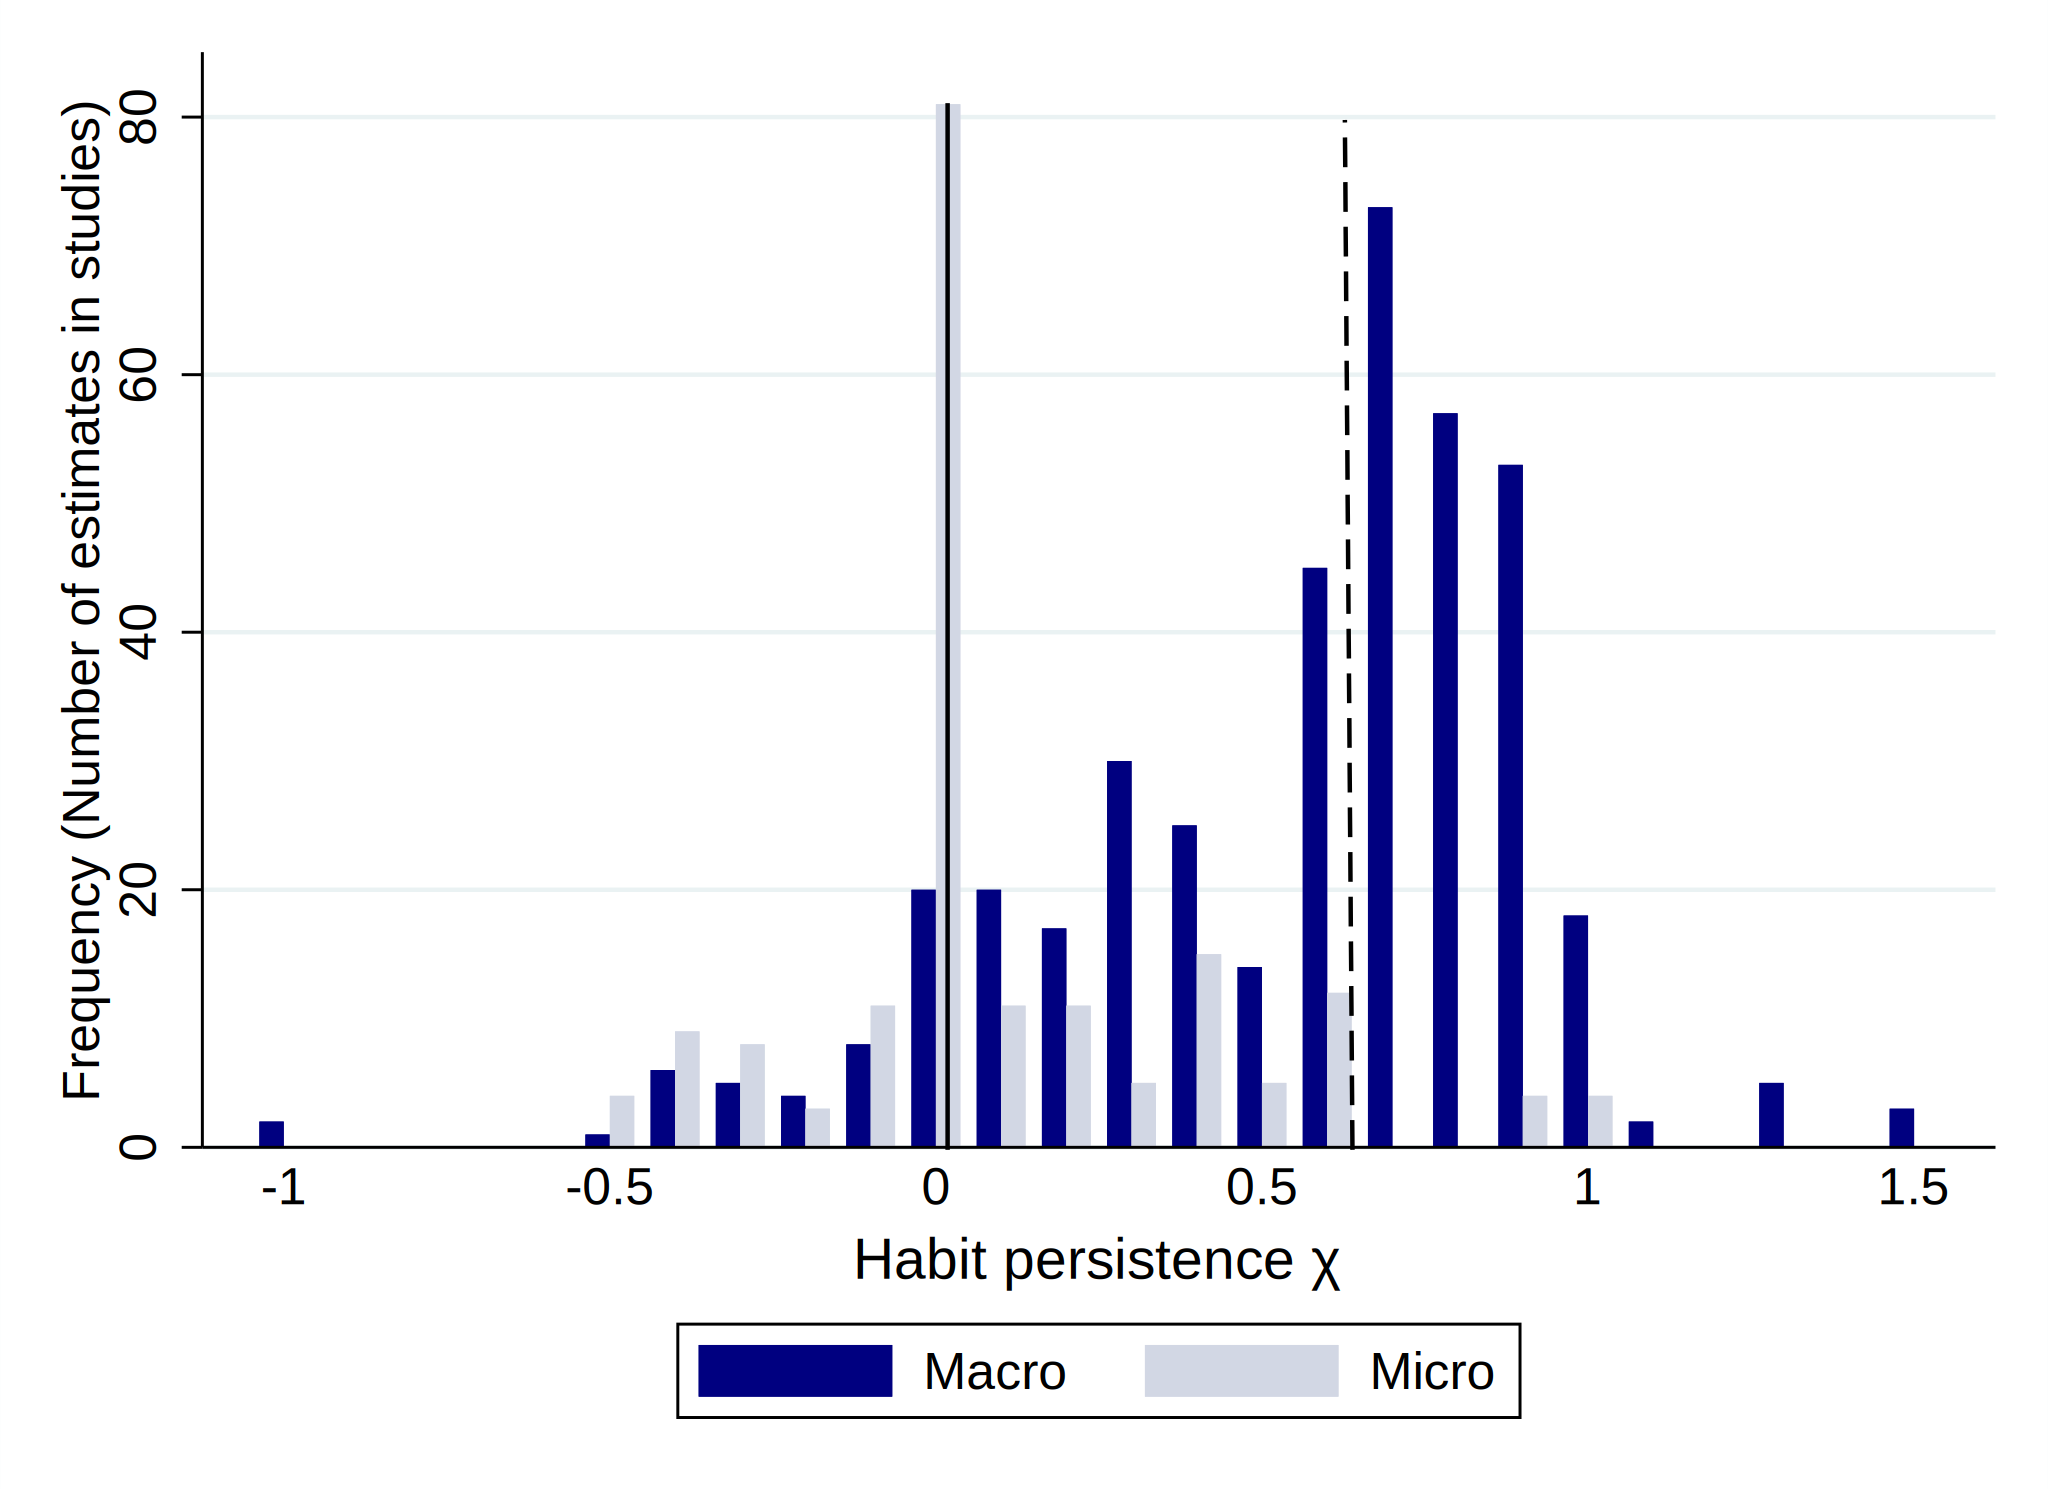
\includegraphics[width=1.5\textwidth]{./Figures/microMacroMetaHistogram}}
    \end{minipage}
      }
{ 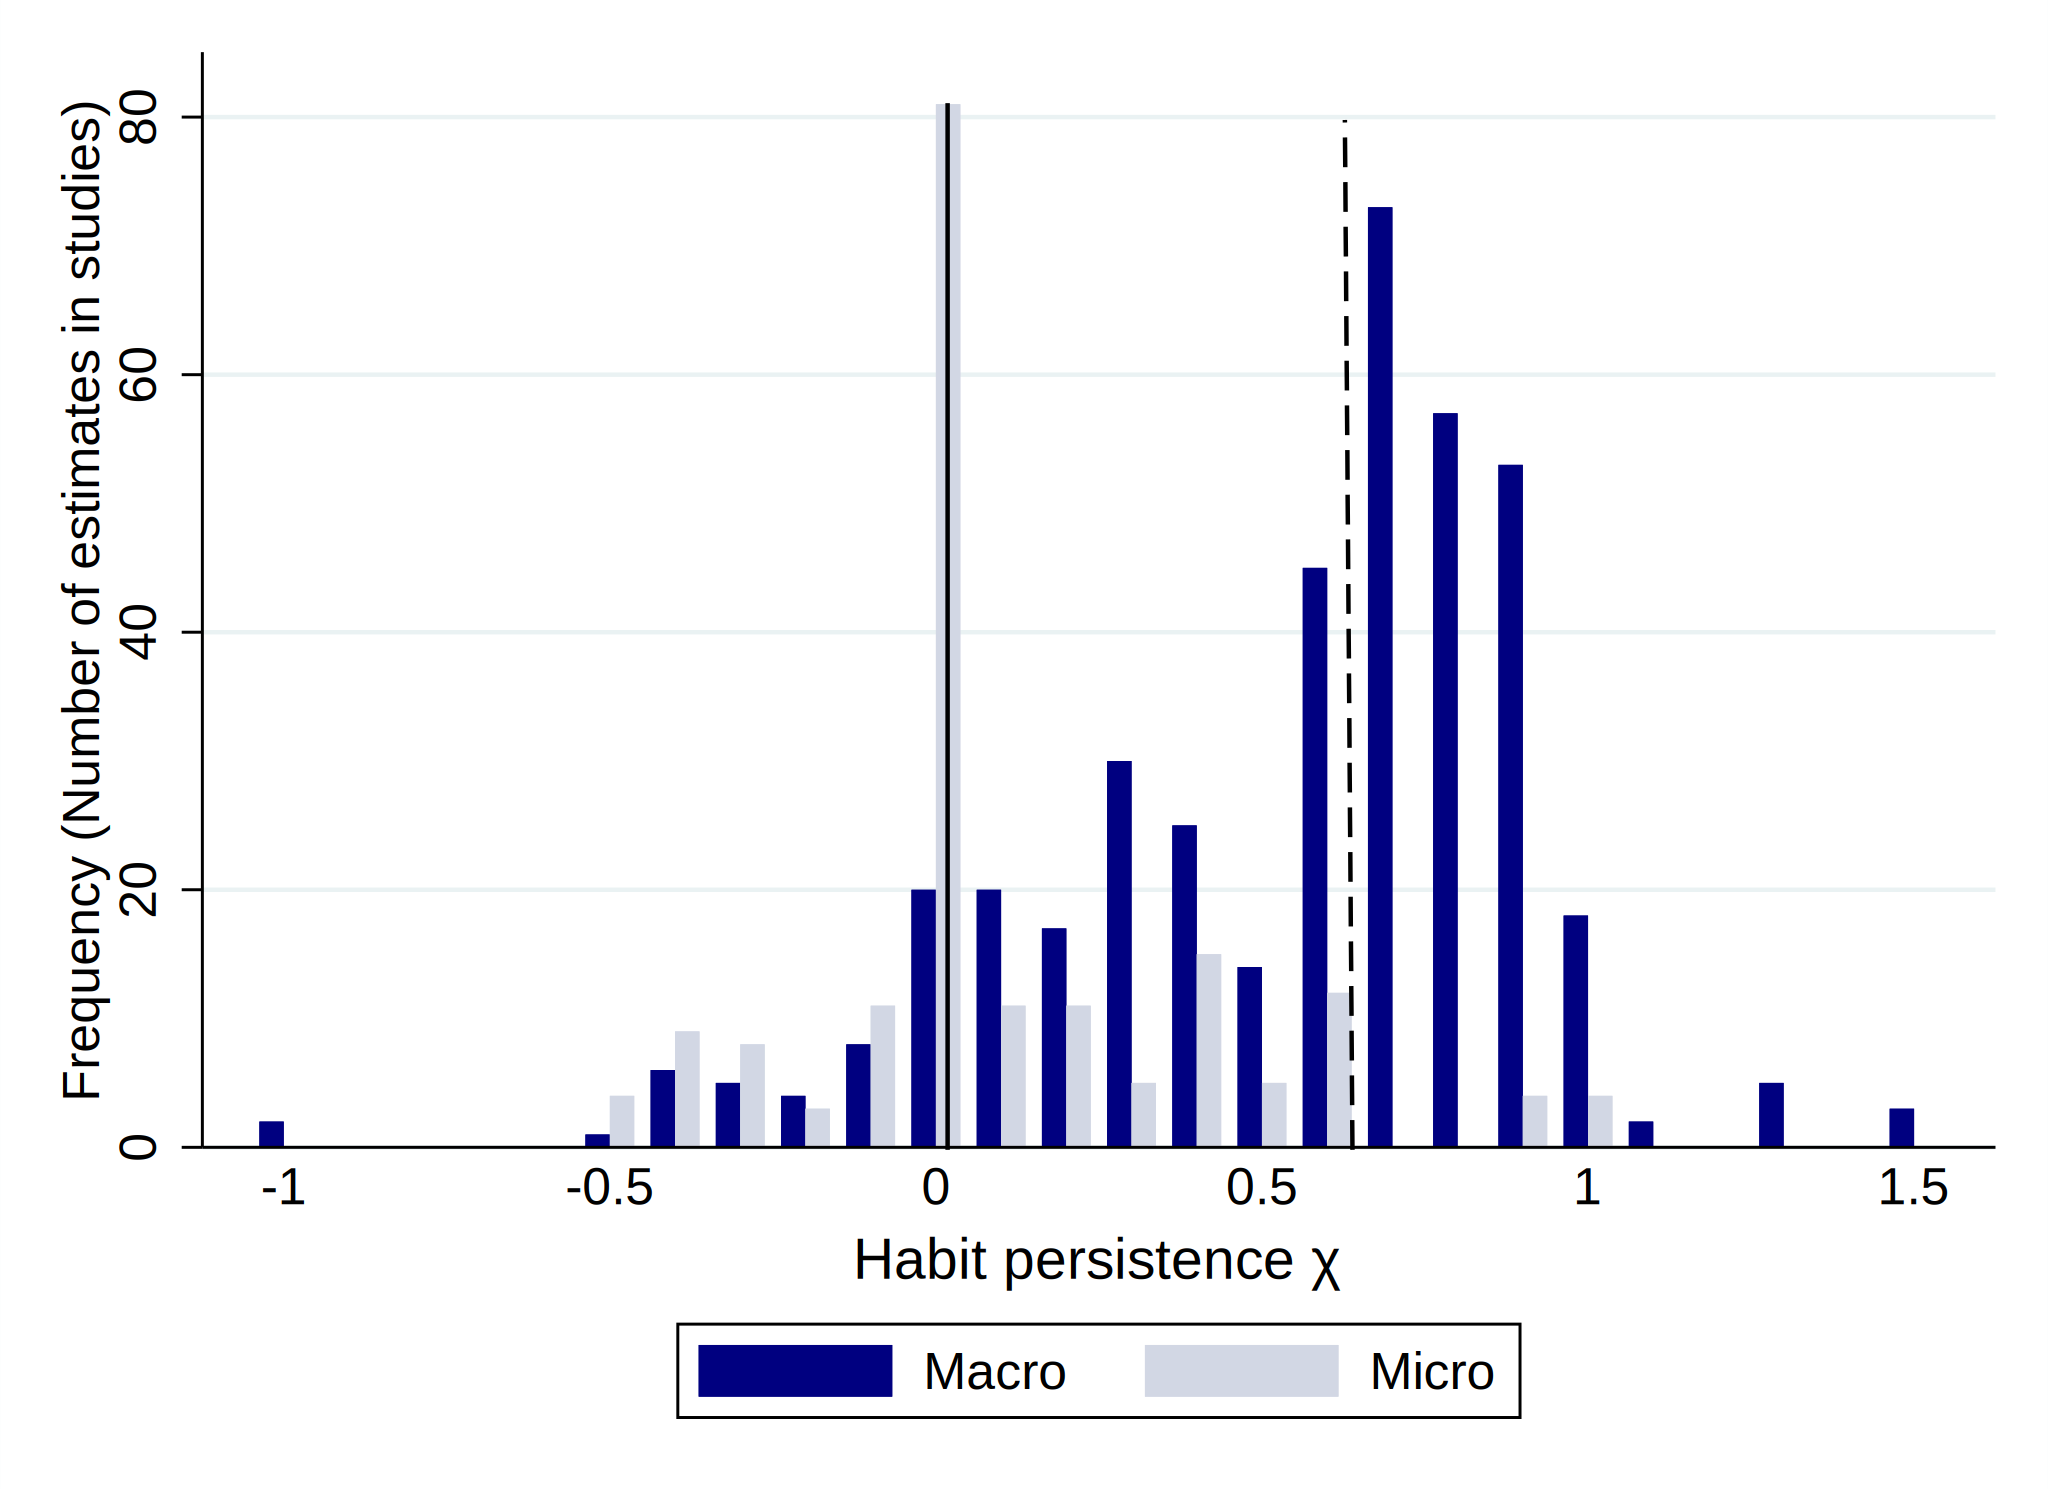
\includegraphics[width=1.0\textwidth]{./Figures/microMacroMetaHistogram}}
\footnotesize Notes: Reproduced from \cite{hrsHabit}, Figure~2. The figure shows the distribution of estimates of habit persistence in studies based on macro and micro data. Solid and dashed lines show the median estimates in micro (0.0) and macro (0.6) studies, respectively.
\end{figure}

If habits are a true structural characteristic of people's utility functions, we should see their effects microeconomic data as well as macroeconomic aggregates.  But empirical studies using household-level data strongly reject the existence of habits of the magnitude necessary to explain aggregate consumption dynamics.  The modal estimate from \cite{hrsHabit}'s survey of the micro literature is a `habit' parameter of 0; the mean estimate is about 0.1 (see Figure~\ref{microMacroMetaHistogram}).\footnote{\cite{dynanHabits} is the best known micro study; many others are reported in \cite{hrsHabit}.  It is well-known that household-level data on consumption are subject to substantial measurement error. Consequently, some attenuation of the micro estimates of $\chi$ might be expected (even though many studies use estimation techniques robust to measurement error). But an extreme amount of noise would be required for the estimated coefficient to be as close to 0 as estimated for the many micro studies in Figure~\ref{microMacroMetaHistogram}.  } Even among studies that have found evidence against the random walk proposition in micro data,\footnote{See the detailed discussion in Section~\ref{subsec:simMicro}.} few claim to have found more than a few percentage points' worth of household-level spending growth to be predictable at any measured horizon.  Roughly speaking, the predictability of aggregate spending growth is around an order of magnitude larger than predictability of household-level spending growth (say, 0.30 versus 0.03 in an adjusted ${R}^{2}$ sense).

We propose a simple solution to this puzzle.  Instead of having consumption habits, microeconomic consumers experience a modest informational friction: Not everybody instantaneously notices all \emph{macroeconomic} developments.  Instead, households' macroeconomic expectations are ``sticky,'' as in \cite{mrSlumps} and~\cite{carroll:epidemicinflQJE}.  Specifically, while each consumer perfectly (`frictionlessly') perceives his own personal circumstances (employment status, wage rate, income received, etc), consumers' information about macroeconomic quantities like aggregate productivity growth arrives only occasionally (as in the Calvo model of firms' price updating).

Consumption sluggishness {\it a la} \cite{cdSmooth} arises as follows.  As in the standard (frictionless) setup, sticky-expectations households perfectly observe their market resources (wealth, debt, etc) and income. However, a consumer whose beliefs about the state of the aggregate economy are out of date will behave in the ways that would have been macroeconomically appropriate (for the consumer's currently observed level of wealth etc) at the time of their last (and possibly out-of-date) perception of macroeconomic circumstances.  The model thus generates a lag in the response of aggregate spending to aggregate developments; the amount of sluggishness will depend on the frequency with which consumers update.  When our model's updating frequency is calibrated to match conventional estimates of the degree of inattention measured using expectations data  on other aggregate variables (e.g., inflation expectations), the model's implications for the persistence in aggregate consumption growth match well the estimates of the `excess smoothness' of consumption growth in the macro literature.

Despite aggregate sluggishness, at the level of individual households, high-frequency consumption growth has little predictability.  This can be reconciled with aggregate smoothness because the rationally appropriate contribution of the consumer's perception of the macroeconomic environment to their individual spending choices is swamped by the importance of fluctuations in idiosyncratic components of income which we assume consumers have no difficulty observing (and to which we assume they are perfectly attentive).\footnote{Over long spans of time---say, over a life cycle---models with uncertainty and impatience imply that consumption growth parallels income growth.  The theory has bite only when applied to high frequency movements in income---say, at the quarterly or annual frequency.}

In our model, the sticky updating of beliefs about the aggregate economy takes the same form (and has the same magnitude) as proposed in~\cite{carroll:epidemicinflQJE} as a microfoundation for the~\cite{mrSlumps} model.  An advantage compared to those papers is that because we are using an optimizing model, we are able to calculate an explicit utility cost of stickiness.  Consistent with a theme in the literature on inattentiveness all the way back to \cite{ayNearRational}, we find that the utility penalty from inattention is low, so that, under our calibrated parameters, our consumers would not be willing to pay much for even the most perfect information about the macroeconomic state:  They would be willing to pay roughly one two-thousandth of their lifetime income to be perfectly informed in every future period of their lifetime.

Our results are essentially the same in a partial equilibrium model (in which factor prices are constant) and a heterogeneous-agents DSGE model with aggregate shocks (which affect factor prices).\footnote{In both environments we calibrate households' income processes to be consistent with evidence from both microeconomic and macroeconomic data.}  Data simulated from our models reproduce what we take to be the main stylized facts about individual and aggregate consumption dynamics.

When estimated on simulated \emph{individual} data (corresponding to microeconomic evidence), regressions in the spirit of \cite{hallRandomWalk} and \cite{cmModel} find that consumption growth exhibits little persistence.  This result is essentially identical across all variants of our models: partial or general equilibrium, with or without inattention. It comports well with the conclusions of a micro literature that was already large when \cite{deatonUnderstandingC} surveyed it and has remained consistent in finding little persistence.  In this respect (and all others), the micro implications of the model are standard for models of this type (with uninsurable uncertainty as well as precautionary saving and perhaps liquidity constraints), which have been extensively studied in the micro literature.\footnote{For example, the model reproduces the robust pattern of evidence since \cite{zeldes:jpe} has documented that consumption growth is faster for people with very low cash-on-hand (who may be near a liquidity constraint or below their desired precautionary buffers---or both).}

We then analyze \cite{hallRandomWalk}/\cite{cmModel} regressions with simulated \emph{aggregate} data. Thanks to the law of large numbers, the idiosyncratic shocks that dominate the household data cancel out upon aggregation, leaving only the residual systematic factors, which generate the much greater predictability in aggregate than in idiosyncratic data.  \cite{cmModel} proposed that such predictability arises because some people just spend all their income, and income growth is predictable.  The habit formation literature has argued instead that predictability reflected the sluggishness of consumption growth itself.  Horserace regressions that pit these two possibilities against each other produce a clear winner: Almost all of the predictability of consumption growth is explained by its correlation with lagged consumption growth; only a small portion comes from the predictable component of aggregate income growth -- both in the data and in our model.

After a brief review of the extensive relevant literature, we begin explaining our ideas with a `toy model' (section~\ref{sec:Quadratic}) in which the key mechanisms can be derived analytically, thanks to extreme simplifying assumptions like quadratic utility and constant factor prices.  We next (section \ref{sec:models}) present the full versions of our models, which abide by the more realistic assumptions (CRRA utility, aggregate as well as individual shocks, time varying factor prices, etc) that have become conventional respectively in the micro and macro literatures.

After calibrating the model (section~\ref{sec:calibration}), we describe the stylized facts from both the micro and macro literatures that we argue need to be explained by a good microfounded macroeconomic model of consumption, and show that all of the various versions of our model (partial versus general equilibrium, etc) robustly reproduce those facts (section \ref{sec:Results}).  This robustness indicates that our results are not a fragile implication of any highly specific framework but instead flow from the underlying structure of inattention that is the common element across all versions of our model (including the quadratic utility `toy model' where the consequences can be seen most clearly).  We then (section \ref{sec:uCost}) calculate how much a fully informed consumer would be willing to pay at birth to enjoy instantaneous and perfect knowledge of aggregate developments as they live their life (not much, it turns out).

With our model's quantitative results in hand, we describe the quantitative and qualitative differences between our model and the other `imperfect information' approaches to explaining aggregate consumption smoothness that have been explored in the prior literature (section \ref{sec:Comparisons}).  Our conclusion suggests directions for future research.



\section{Relation to the Literature}\label{sec:relation}

No review of the empirical literature is needed; \cite{hrsHabit} have done an admirable job.  Our only critique is that they have followed much of the prior literature in casually referring to the parameter of interest as the `habit coefficient.'  A better choice would have been to call it the `excess smoothness' coefficient; ours is not the first paper to suggest that habits are not the only possible explanation for why consumption growth might be too smooth (compared to the \cite{hallRandomWalk} benchmark).

Our `sticky expectations' approach is related to several strands of the burgeoning literature on models of imperfect information processing.  A major strand in that literature is models of `rational inattention' in the spirit of \cite{simsInattention}, in which agents have a limited ability to pay attention and allocate it optimally, recently embodied (for example) in the work of \cite{mackWiedREStud15}.  They study a DSGE model with inattentive consumers and firms using a simple New Keynesian framework in which they replace all sources of slow adjustment (habit formation, Calvo pricing and wage setting) with rational inattention.  The setup with rational inattention can match the sluggish responses observed in aggregate data, in response both to monetary policy shocks and to technology shocks.

A challenge to this approach has been the extraordinary complexity of solving models that aim to work out the full implications of the fact that everyone else is working out the full implications of the fact that everyone else is rationally inattentive.\footnote{For example, the literature on rational inattention has adopted a more stylized setup of idiosyncratic and aggregate income shocks and, to our knowledge, has so far not solved the full \cite{ksHetero} framework.}
In response, \cite{gabaixSparsityQJE} has recently proposed a framework that is much simpler than the full rational inattention framework of \cite{simsInattention}, but aims to capture much of its essence.  This approach is relatively new, and while it does promise to be more tractable than the full-bore Simsian rational inattention framework, even the simplified Gabaix approach would be formidably difficult to embed in a model with a rich treatment of transitory and persistent income shocks, precautionary motives and other complexities entailed in modern models of microeconomic consumption decisions. It would be similarly challenging to determine how to apply the approaches of \cite{woodfordImperfect} or \cite{msInertiaAER} to our question.\footnote{Arguably, our Calvo-style updating is not too different from what one might get in a suitably adapted version of the \cite{msInertiaAER} model.}

Another way to dial back the complexity of the rational inattention approach is to radically simplify the model's assumptions about decisionmaker's problem.  In that spirit \cite{reis:inattentive} considers a model in which consumers with a linear consumption function and a conveniently simple environment optimally choose to be inattentive because of explicit (fixed monetary) costs of attention.\footnote{\cite{reis:inpro} presents a similar setup with a producer setting prices subject to information processing constraints.}  In this framework, \cite{reis:inattentive} is able to calculate an explicit analytical formula for the tradeoff between the disutility from the increase in uncertainty caused by inattention, and the monetary savings due to infrequent payment of the cost of information.  Reis shows that in his model, inattention is manifested in the fact the his consumers only gather new information (and therefore only update their consumption) at fixed intervals whose length depends on the cost of obtaining information versus the costs of remaining ignorant.

One of our objectives is to faithfully match microeconomic data.  In such data there is incontrovertible evidence---most recently from millions of datapoints from the Norwegian population registry examined by \cite{fhnMPC}---that the consumption function is not linear.  It is concave, as the general theory suggests (\cite{carroll&kimball:concavity}), and this concavity matters greatly for matching the main micro facts.  There is also nothing that looks  either like the Reis model's prediction that there will be extended periods in which consumption does not change at all, nor its prediction that there will be occasional periods in which it moves a lot (at dates of adjustment) and then remains constant at that newer level for some extended period.  This critique applies generically to models that incorporate a convex cost of adjustment---whether to the consumer's stock of information (\cite{reis:inattentive}) or to the level of consumption as in \cite{chettySzeidl:cCommitmentsEcta}.  All such models imply counterfactually `jerky' behavior of spending at the microeconomic level.\footnote{This pattern {\it does} match consumers' purchases of durable goods like automobiles; but the `excess smoothness' facts hold as strongly for aggregate nondurables as for durable goods.  The fixed-adjustment-cost framework matches many other economic decisions well---for instance, individual investors adjust their portfolios sporadically even though the prices of many assets experience large fluctuations at high frequency---and \cite{alvarezGuisoLippi:DurCons} find ``a robust pattern consistent with the assumption that a component of adjustment costs is information gathering'' (p.~2273).}

To better match the micro data, we use the now-conventional microeconomic formulation in which utility takes the Constant Relative Risk Aversion form and uncertainty is calibrated to match micro estimates.  Our assumption that consumers can perfectly observe the idiosyncratic components of their income allows us to use essentially the same solution methods as in the substantial recent literature exploring models of this kind; our assumption that macroeconomic expectations are sticky makes no material difference to the solution of the model.\footnote{A fascinating study that does not fit neatly into this analysis is~\cite{jpsTax}, who show that spending in the U.S.  responded strongly to the random idiosyncratic variation in the timing of tax refunds.  Their results might possibly be consistent with a model in which households can see the contents of their bank accounts but do not pay attention to tax policy, which has the flavor of the model proposed here. Similarly, \cite{Kueng:Near-rationality} argues that excess sensitivity of consumption is consistent with households following near-rational plans and that to model macroeconomic policies, such as economic stimulus programs, near-rational alternatives can perform better than standard consumption models.
}  Implementing the state of the art in the micro literature adds a great deal of complexity and precludes a closed form solution for consumption like the one used by Reis; its virtue is that the model is quantitatively plausible enough that, for example, it might actually be usable by policymakers who wanted to assess the likely dynamics entailed by alternative fiscal policy options.

Given our choice to embrace the challenge of matching micro data, it was essential to keep the rest of the model as simple as possible, in the spirit of \cite{ayNearRational}, \cite{cochrane:nearrational}, \cite{mrSlumps} and as forcefully advocated by \cite{browning&crossley:lifecycle}. In pursuit of such simplicity, we adopt the  \cite{calvoPrices}-like framework of \cite{carroll:epidemicinflQJE} in which updating is a Poisson event.\footnote{\cite{BrowningColladoAER} speculate that the differing results in the micro literature can be resolved if consumers are not perfectly attentive even to all the details of their own personal income processes, an explanation which could easily be interpreted using framework proposed here.}

Inattention is not the only alternative to habits as an explanation for excess smoothness.  Information itself can be imperfect, even for a perfectly attentive consumer.  The seminal work contemplating this possibility was by \cite{muthOptimal}, whose most direct descendant in the consumption literature is \cite{pischkeMicroMacro} (building also on \cite{lucas:imperfectInfo}).  The idea is that (perfectly attentive) consumers face a signal extraction problem in determining whether a shock to income is transitory or permanent.  When a permanent shock occurs, the immediate adjustment to the shock is only partial, since agents' best guess is that the shock is partly transitory and partly permanent.   With the right calibration, such a model could in principle explain any amount of excess smoothness.  But we argue that when a model of this kind is calibrated to the actual empirical data, it generates only a modest amount of excess smoothness, far less than exhibited by the empirical data.

Moving from theory to evidence, there is an interesting and growing literature that uses expectations data from surveys in an attempt to directly measure sluggishness in expectations dynamics.\footnote{We omit a fuller survey of this interesting literature because expectations data will not be our focus here.} For example, \cite{coibGor:AER15} find that the implied degree of information rigidity in inflation expectations is high, with an average duration of six to seven months between information updates. \cite{fuhrer:JME17} and \cite{fuhrer:IntrinsicPersistence} find that even for professional forecasters, forecast revisions are explainable using lagged information, which would not be the case under perfect information processing.



\section{A Quadratic Utility `Toy Model'}\label{sec:Quadratic}

Here we briefly introduce concepts and notation, and motivate the key result using a simple framework with quadratic utility.  We start with the classic \cite{hallRandomWalk} random walk model, with the standard assumption of time separable utility and geometric discounting by factor $\beta$.  Overall wealth $\wAllLev$ (the sum of human and nonhuman wealth) evolves according to the dynamic budget constraint
\begin{verbatimwrite}{\eq/zAccum.tex}
\begin{eqnarray}
  \wAllLev_{t+1} & = & (\wAllLev_{t}-\cLevBF_{t})\Rfree+\zeta_{t+1}, \label{eq:zAccum}
\end{eqnarray}
\end{verbatimwrite}
\input \eq/zAccum.tex
where $\Rfree=(1+\rfree)$ is the interest factor and $\zeta_{t+1}$ is a shock to (total) wealth.

With no informational frictions, the usual derivations lead to the standard Euler equation:
\begin{verbatimwrite}{\eq/QuadEuler.tex}
\begin{eqnarray*}
  \uFunc^{\prime}(\cLevBF_{t}) & = & \Rfree\beta \Ex_{t}\big[\uFunc^{\prime}(\cLevBF_{t+1})\big], \label{eq:QuadEuler}
\end{eqnarray*}
\end{verbatimwrite}
\input \eq/QuadEuler.tex
where $\Ex_{t}$ denotes an assumption of instantaneous perfect frictionless updating of all information. Quadratic $\uFunc$ and $\Rfree \beta=1$ imply Hall's random walk proposition:
\begin{verbatimwrite}{\eq/dCQuad.tex}
\begin{eqnarray*}
  \Delta \cLevBF_{t+1} & = & \varepsilon_{t+1} \label{eq:dCQuad}.
\end{eqnarray*}
\end{verbatimwrite}
\input \eq/dCQuad.tex
Consumers spend
\begin{eqnarray*}
  \cLevBF_{t} & = & (\rfree/\Rfree) \wAllLev_{t}, \label{eq:cquad}
\end{eqnarray*}
because this is exactly the amount that maintains expected wealth unchanged:
\begin{eqnarray*}
  \Ex_{t}[\wAllLev_{t+1}] & = & (\wAllLev_{t}-\cLevBF_{t})\Rfree = \wAllLev_{t}
%\\ \ifnumSw \wAllLev_{t+1} & = & \wAllLev_{t}+\zeta_{t+1}
.
\end{eqnarray*}


\subsubsection*{Sticky Expectations}

Now suppose consumers update their information about $\wAllLev_t$, and therefore their behavior, only occasionally.  A consumer who updates in period $t$ obtains precisely the same information that a consumer in a frictionless model would receive, forms the same expectations, and makes the same choices.  Nonupdaters, however, behave as though their former expectations had actually come true (since by definition these are the persons who have learned nothing to disconfirm their prior beliefs).  For example, consider a consumer who updates in periods $t$ and $t+n$ but not between.  Designating $\perc{\wAllLev}$ as the consumer's {\it perception} of wealth:
  \begin{eqnarray*}
\perc{\wAllLev}_{t+j} & \equiv & \Ex_{t}[\wAllLev_{t+j}] = \wAllLev_{t} \qquad \text{for }  1\le j < n,
\end{eqnarray*}
  the consumer spends according to perceived wealth so that
  \begin{eqnarray*}
\cLevBF_{t+j} & = & (\rfree/\Rfree)\perc{\wAllLev}_{t+j} = (\rfree/\Rfree)     \wAllLev _{t} = \cLevBF_{t} \qquad \text{for }  1\le j < n.
\end{eqnarray*}
The dynamics of actual (as distinct from perceived) wealth are given by \eqref{eq:zAccum},
\begin{verbatimwrite}{\eq/zt.tex}
\begin{eqnarray*}
        \wAllLev_{t+1} & = & \overbrace{\wAllLev_{t}}^{=\,(\wAllLev_{t}-\cLevBF_{t})\Rfree}+\zeta_{t+1}  \\
        \wAllLev_{t+2} & = & \wAllLev_{t+1}+\zeta_{t+2}=\wAllLev_{t}+\zeta_{t+1}\Rfree + \zeta_{t+2}
%        \wAllLev_{t+3} & = & \wAllLev_{t}+\Rfree^{2} \epsilon_{t+1} + \Rfree \epsilon_{t+2}
\\ \vdots       &   & \vdots \nonumber
\\  \wAllLev_{t+n} & = & \wAllLev_{t}+\underbrace{\sum_{s=1}^{n} \Rfree^{n-s}\zeta_{t+s}}_{\equiv\,\Delta^{n} \wAllLev_{t+n}},
\end{eqnarray*}
\end{verbatimwrite}
\input \eq/zt.tex
so for a consumer who updates in periods $t$ and $t+n$ but not between, the change in consumption is
\begin{verbatimwrite}{\eq/ctpnMct.tex}
\begin{eqnarray*}
\ifnumSw        \cLevBF_{t+n}-\cLevBF_{t}  & = & (\rfree/\Rfree)\Delta^{n}\wAllLev_{t+n},
\end{eqnarray*}
\end{verbatimwrite}
\begin{eqnarray*}
\ifnumSw        \cLevBF_{t+n}-\cLevBF_{t}  & = & (\rfree/\Rfree)\Delta^{n}\wAllLev_{t+n},
\end{eqnarray*}
 where $\Delta^{n}\wAllLev_{t+n}$ is white noise because it is a weighted sum of the white noise errors $\zeta$.  Thus, consumption follows a random walk across updating periods; consumers who were only observed during their updating periods would never be seen to deviate from the predictions of \cite{hallRandomWalk}.


\subsubsection*{Aggregation}

The economy is populated by consumers indexed by $i$, distributed uniformly along the unit interval.  Aggregate (or equivalently, per capita) consumption is
\begin{verbatimwrite}{\eq/CAgg.tex}
\begin{eqnarray*}
        \CLevBF_{t} & = & \int_{0}^{1} \cLevBF_{t,i}\,\text{d}i
\ifslides{}{.}
\end{eqnarray*}
\end{verbatimwrite}
\input \eq/CAgg.tex

Whether the consumer at location $i$ updates in period $t$ is determined by the realization of the binary random variable $\pi_{t,i}$, which takes the value 1 if consumer $i$ updates in period $t$ and 0 otherwise.  Each period's updaters are chosen randomly such that a constant proportion $\Pi$ update in each period:
\begin{eqnarray*}
   \Ex[\pi_{t+1,i}] &= & \Pi \qquad \forall\,t \text{ and } i,
\\ \int_{0}^{1} \pi_{t,i}\,\text{d}i & = & \Pi \qquad \forall\,t
\ifslides{}{.}
\end{eqnarray*}

Aggregate consumption is the population-weighted average of per-capita consumption of updaters $\CLevBF^{\pi}$ and nonupdaters $\CLevBF^{\cancel{\pi}}$:
\begin{eqnarray}
 \CLevBF_{t+1} & = & \Pi \CLevBF^{{\pi}}_{t+1}+(1-\Pi) \underbrace{\CLevBF^{\cancel{{\pi}}}_{t+1}}_{=\,\CLevBF_{t}}, \label{eq:Ctp1}
\end{eqnarray}
where per-capita consumption $\CLevBF^{\cancel{{\pi}}}_{t+1}=\CLevBF_{t}$ because the
nonupdaters at time $t+1$ are a random subset of the population at time $t$.
The first difference of \eqref{eq:Ctp1} yields
\begin{eqnarray*}
  \Delta \CLevBF_{t+1} & = &  (1-\Pi) \Delta \CLevBF_{t} + \underbrace{\Pi \Delta \CLevBF^{{\pi}}_{t+1}}_{\equiv\,\varepsilon_{t+1}} \label{eq:deltac} \label{eq:dCQuadStickyApprox}
\end{eqnarray*}
and Appendix~\ref{appendix:QuadCDyn} shows that $\varepsilon_{t+1}$ is approximately mean zero.\footnote{Intuitively, this term mainly reflects the behavior of updating consumers, and is therefore unpredictable with respect to sufficiently delayed information.}  Thus, in the quadratic utility framework the serial correlation of aggregate per-capita consumption changes is an approximate measure of the proportion of nonupdaters.

This is the mechanism behind the exercises presented in Section \ref{sec:Results}.  While the details of the informational friction is different in the more realistic models we will set up in Section \ref{sec:models}, the same logic and quantitative result holds: the serial correlation of consumption growth approximately equals the proportion of non-updaters.

Note further that the model does {\it not} introduce any explicit reason that consumption growth should be related to the predictable component of income growth {\it a la} \cite{cmModel}.  In a regression of consumption growth on the predictable component of income growth (and nothing else), the coefficient on income growth would entirely derive from whatever correlation predictable income growth might have with lagged consumption growth.  This is the pattern we will find below, both in our theoretical and our empirical work.



\section{Real Models}
\label{sec:models}

One of the lessons of the consumption literature after \cite{hallRandomWalk} is that his simplifying assumptions (quadratic utility, perfect capital markets, $\Rfree\beta=1$) are far from innocuous; more plausible assumptions can lead to very different conclusions.  In particular, a host of persuasive theoretical and empirical considerations has led to the now-standard assumption of constant relative risk aversion utility, $\uFunc(\cLevBF)=\cLevBF^{1-\CRRA}/(1-\CRRA).$ When utility is not quadratic, solution of the model requires specification of the exact stochastic structure of the income and transition processes.

Below, we present two models that will be used to simulate the economy under frictionless and sticky expectations.  First, we specify a small open economy (or partial equilibrium) model with a rich and empirically realistic calibration of idiosyncratic and aggregate risk but exogenous interest rates and wages. Second, we extend the SOE model to a heterogeneous agents dynamic stochastic general equilibrium (closed-economy) model that endogenizes factor returns, at the cost of a more burdensome computational task.\footnote{Appendix \ref{sec:RepAgent} presents a model that abstracts from idiosyncratic income risk (essentially, setting $\sigma^{2}_{\psi}=\sigma^{2}_{\theta}=0$), and which produces results similar to those of our `realistic' models.  The simplification enables general equilibrium analysis at a small fraction of the computational cost. However, it is neither a recognizable representative agent model nor a respectable heterogeneous agents model, which may reduce its appeal to both audiences.}

\subsection{General Modeling Assumptions}
\label{section:Models}

Several features are common across all our models.  A continuum of agents care about expected lifetime utility derived from CRRA preferences over a unitary consumption good; they geometrically discount future utility flows by discount factor $\beta$.  These agents inelastically supply one unit of labor, and their only decision in each period $t$ is how to divide their market resources $\mLevBF$ between consumption $\cLevBF$ and saving in a single asset $\aLevBF$.  We assume agents are \cite{blanchardFinite} ``perpetual youth'' consumers: They have a constant probability of death $\PDies$ between periods, and upon death they are are immediately replaced, while their assets are distributed among surviving households in proportion to the recipient's wealth.

\subsubsection{Output, Income, and Productivity}

Output is produced by a Cobb--Douglas technology using capital $\KLevBF_t$ and (effective) labor $\LLevBF_t$; capital depreciates at rate $\delta$ immediately after producing output, leaving portion $\daleth=1-\delta$ intact, and as usual the effectiveness of labor depends on the level of aggregate labor productivity.

We represent both aggregate and idiosyncratic productivity levels as having both transitory and permanent components.  Large literatures have found that this representation is difficult to improve upon much in either context, and the simplicity of this description yields considerable benefits both in the tractability of the model, and in making its mechanics as easy to understand as possible.

In more detail, aggregate permanent labor productivity $\PLev_t$ grows by factor $\PtyGro_t$, subject to mean one iid aggregate permanent shocks $\Psi_t$, so the aggregate productivity state evolves according to:
\begin{equation}
{\PLev}_{t+1} = \PtyGro_{t+1} {\PLev}_{t}\Psi_{t+1}, \text{ where} \qquad\text{Prob}[\PtyGro_{t+1}=\PtyGro_k | \PtyGro_t = \PtyGro_j] = \Xi_{j,k}.   \label{eq:AggRandWalk}
\end{equation}
The productivity growth factor $\PtyGro_t$ follows a bounded random walk, as in (for example) \cite{edge2007Learning}, which is part of a literature whose aim is to capture in a simple statistical way the fact that underlying rates of productivity growth seem to vary substantially over time (e.g., fast in the 1950s, slow in the 1970s and 1980s, moderate in the 1990s, and so on; see also \cite{jorgenson:ProductivityGrowthResurgence}).\footnote{We capture the process by discretizing the range of productivity growth rates within our bounds, and calibrate the Markov transition probability matrix $\Xi$ so that the statistical properties of productivity growth rates exhibited by our process match the corresponding properties measured in U.S.\ data since the 1950s.}  We introduce these slow-moving productivity growth rates not just for realism but also because we need to perform, in our simulated data, exercises like those \cite{cmModel} performed in empirical data, in which consumption growth is regressed on the component of income growth that was predictable using data lagged several quarters.  We therefore need a model in which there {\it is} some predictability in income growth several quarters in the future.

The transitory component of productivity in any period is represented by a mean-one variable $\Theta_t$, so the overall level of aggregate productivity in a given period is $\PLev_{t}\Theta_{t}$.

Similarly, each household has an idiosyncratic labor productivity level $p_{t,i}$, which (conditional on survival) evolves according to:
\begin{equation}
p_{t+1,i} = p_{t,i} \psi_{t+1,i},  \label{eq:IndRandWalk}
\end{equation}
and like their aggregate counterparts, idiosyncratic permanent productivity shocks are mean
one iid ($\Ex_{t}[\psi_{t+n,i}]=\Ex_{t}[\Psi_{t+n}]= 1~\forall ~n>0$).\footnote{Because we did not have any modeling purpose for which we needed a slow-moving persistent component to idiosyncratic productivity growth, we omitted it.  If we wanted a completely parallel representation of the aggregate and idiosyncratic processes, we could introduce a term $\ptyGro_{t,i} \equiv 1 ~\forall~t$.}
Total labor productivity for the individual is determined by the interaction of transitory idiosyncratic
($\theta$), transitory aggregate ($\Theta$), permanent idiosyncratic $({p})$, and permanent aggregate
$({P})$ factors.  When the household supplies one unit of labor, this contributes effective labor equal to:
\begin{verbatimwrite}{\eq/ell.tex}
\newcommand{\TranShocktpOne }{\Theta_{t}}
\begin{eqnarray}
  \label{eq:ell}
\ifnumSw  \pmb{\ell}_{t,i} & = & \overbrace{\theta_{t,i}\TranShocktpOne}^{\equiv\,\pmb{\theta}_{t,i}}\underbrace{{p}_{t,i} {P}_{t}}_{\equiv\,\pLev_{t,i}}.
\end{eqnarray}
\end{verbatimwrite}
\newcommand{\TranShocktpOne }{\Theta_{t}}
\begin{eqnarray}
  \label{eq:ell}
\ifnumSw  \pmb{\ell}_{t,i} & = & \overbrace{\theta_{t,i}\TranShocktpOne}^{\equiv\,\pmb{\theta}_{t,i}}\underbrace{{p}_{t,i} {P}_{t}}_{\equiv\,\pLev_{t,i}}.
\end{eqnarray}
 Here, $\theta$ can be thought of as reflecting, for example, individual unemployment spells, while $\Theta$ captures, e.g., disruptions in output due to bad weather.  Just like aggregate transitory shocks, $\theta_{t,i}$ is mean one and iid, so that $\Ex_{t}[\theta_{t+n,i}]=\Ex_{t}[\Theta_{t+n}]=1~\forall~n>0$.  \ifZero{ The idiosyncratic transitory shock has a minimum possible value of 0 (corresponding to an unemployment spell) which occurs with a small finite probability $\pZero$.  This has the effect of imposing a `natural borrowing constraint' (cf.\ \cite{zeldesStochastic}) at zero.}{}

\subsubsection{Perceptions and Behavior}

For understanding the decisions of an individual consumer in a frictionless (i.e., perfect information) world the aggregate and idiosyncratic transitory shocks can be combined into a single overall transitory shock indicated by the boldface $\pmb{\theta}$, and the aggregate and idiosyncratic levels of permanent income can be combined as $\pLev$ (likewise, the combined permanent shock is boldface $\pmb{\psi}_{t,i}\equiv \psi_{t,i} \Psi_{t}$).  However, a key feature of the models used here is that a household does not necessarily know the true value of the aggregate productivity state variables $(\PLev_t,\PtyGro_t)$, as they might not have (stochastically) observed it in the current period.  Instead, each household has \textit{perceptions} about the aggregate state $(\perc{\PLev}_{t,i},\perc{\PtyGro}_{t,i})$.  Our key behavioral assumption is twofold:
\begin{enumerate}
\item Household agents always act \textit{as if} their perception of the aggregate state $(\perc{\PLev}_{t,i},\perc{\PtyGro}_{t,i})$ were the true aggregate state $(\PLev_t,\PtyGro_t)$.

\item Households form their perception of the aggregate state according to the \textit{expectation} of today's state given the last observed aggregate state.
\end{enumerate}
Given the assumption that productivity growth $\PtyGro_t$ follows a random walk,
the second part of the behavioral assumption says that an agent who last observed the true
aggregate state $n$ periods ago perceives:
\begin{equation}\label{eq:PLevBelief}
(\perc{\PLev}_{t,i},\perc{\PtyGro}_{t,i}) = \Ex_{t-n}\big[(\PLev_t,\PtyGro_t) \big| (\PLev_{t-n},\PtyGro_{t-n})\big] = (\PtyGro_{t-n}^n \PLev_{t-n},\PtyGro_{t-n}).
\end{equation}
That is, our assumed random walk in productivity growth means that the household believes that aggregate productivity has grown at the last observed growth rate for the past $n$ periods.\footnote{Because of the boundedness of the random walk in productivity growth, this holds only approximately.}  For households who observed the true aggregate state this period, $n=0$ and thus \eqref{eq:PLevBelief} says that $(\perc{\PLev}_{t,i},\perc{\PtyGro}_{t,i}) = (\PLev_t,\PtyGro_t)$.  The household perceives that their overall permanent productivity level is $\perc{\pLev}_{t,i} = p_{t,i} \perc{\PLev}_{t,i}$.

Households in our models always correctly observe the \textit{level} of all real variables---they are able to read their bank statement and paycheck. But (as will be shown below) consumers' optimal behavior in the frictionless model depends on the {\it ratios} of those real variables to productivity.  That is, for some state variable $\textbf{x}$ (like market wealth), the optimal choice would depend on ${x} \equiv \mathbf{x}/{\pLev}$, where our definition of nonboldface ${x}$ reflects our notational convention that when a level variable has been normalized by the corresponding measure of productivity, it loses its boldness.  The same applies for aggregate variables ${X} \equiv \mathbf{X}/{\PLev}$.

When a household's perception of productivity $\perc{\pLev}$ differs from actual productivity, we denote the perceived ratio as, e.g., $\perc{x} \equiv \mathbf{x}/\perc{\pLev} = \mathbf{x}/({p}\perc{\PLev})$ where the last equality reflects our assumption that the household perceives the idiosyncratic component of their productivity ${p}$ without error.

The behavior of a `sticky expectations' consumer thus differs from that of a frictionless consumer only to the extent that the `sticky expectations' consumer's perception of aggregate productivity is out of date.

\subsubsection{Transition Dynamics}

Infinitely-lived households with a productivity process like \eqref{eq:IndRandWalk} would generate a nonergodic distribution of idiosyncratic productivity---as individuals accumulated ever more shocks to their permanent productivities, those productivities would spread out indefinitely with time. To avoid this inconvenience, we make the \cite{blanchardFinite} assumption: Each consumer faces a constant probability of mortality of $\PDies$ (with complementary survival probability $\PLives$). %15:09 2018/02/03 KT: I have not touched but referees often prefer using (1-$\PDies$) to $\PLives$ because $\PLives$ gives nonstandard notation
We track death events using a binary indicator:
\begin{equation*}
\pDies_{t+1,i} =
  \begin{cases}
    0 & \text{if consumer at location $i$ survives from time $t$ to $t+1$}
\\ \ifnumSw  1 & \text{if consumer at location $i$ dies between $t$ and $t+1$}.
  \end{cases}
\end{equation*}
We refer to this henceforth as a `replacement' event, since the consumer who dies is replaced by an unrelated newborn who happens to inhabit the same location on the number line.  The {\it ex ante} probability of death is identical for each consumer, so that the aggregate mass of consumers who are replaced is time invariant at $\PDies = \int_{0}^{1} \pDies_{t,i}\,\text{d}i$.

Under the assumption that `newborns' have the population average productivity level of $1$, the population mean of the idiosyncratic component of permanent income is always $\int_{0}^{1} {p}_{t,i}\,\text{d}i = 1$.\footnote{The dynamics and steady state of the population variance of the idiosyncratic component of permanent income $\pRat$ are derived in Appendix~\ref{appendix:pss}.  The variance will exist so long as $\PLives \Ex[\psi^{2}] < 1$, which imposes a loose restriction on the magnitude of the idiosyncratic permanent shocks.}  Our earlier equation \eqref{eq:IndRandWalk} for the idiosyncratic productivity transition rule for the inhabitant of location $i$ on the number line is thus adjusted to:\footnote{The constant population size permits the analytical convenience of replacing the dying with newborns, but it is important to understand that there is no relationship between successive persons at the same location on the number line; this is not a dynastic model.}
\begin{verbatimwrite}{\eq/pBlanchard.tex}
\begin{equation*} \ifnumSw
{p}_{t+1,i} =
  \begin{cases}
    \ifnumSw  {p}_{t,i} \psi_{t+1,i} & \text{if } \pDies_{t+1,i} = 0 \\
    1 & \text{if } \pDies_{t+1,i} = 1. \\
  \end{cases}
\end{equation*}
\end{verbatimwrite}
\input \eq/pBlanchard.tex

Along with its productivity level, the household's primary state variable when the consumption decision is made is the level of market resources $\mLevBF_{t,i}$, which captures both current period labor income $\yLevBF_{t,i}$ (the wage rate times the household's effective labor supply) and the resources that come from the agent's capital stock $\kLevBF_{t,i}$ (the value of the capital itself plus the value of the capital income it yields):
\begin{verbatimwrite}{\eq/mDef.tex}
\begin{equation}
\ifnumSw \mLevBF_{t,i} = \underbrace{{\bf \Wage}_{t} \pmb{\ell}_{t,i}}_{\equiv\,\yLevBF_{t,i}} + \underbrace{{\Rprod}_t}_{\daleth+\rfree_{t}} \kLevBF_{t,i}.
\label{eq:mDef}
\end{equation}
\end{verbatimwrite}
\input \eq/mDef.tex
The transition process for $\mLevBF$ is broken up, for convenience
of analysis, into three steps.  `Assets' at the end of the period are
market resources minus consumption:
\begin{verbatimwrite}{\eq/aDef.tex}
\begin{eqnarray}
   \aLevBF_{t,i} & = & \mLevBF_{t,i}-\cLevBF_{t,i}. \label{eq:aDef}
\end{eqnarray}
\end{verbatimwrite}
\input \eq/aDef.tex
Next period's capital is determined from this period's assets via
\begin{verbatimwrite}{\eq/tontine.tex}
\begin{equation*} \ifnumSw
\kLevBF_{t+1,i}  =
\begin{cases}
    \aLevBF_{t,i} /\PLives & \text{if } \pDies_{t+1,i} = 0 \\
     0                       & \text{if } \pDies_{t+1,i} = 1,
\end{cases} \label{eq:tontine}
\end{equation*}
\end{verbatimwrite}
\begin{equation*} \ifnumSw
\kLevBF_{t+1,i}  =
\begin{cases}
    \aLevBF_{t,i} /\PLives & \text{if } \pDies_{t+1,i} = 0 \\
     0                       & \text{if } \pDies_{t+1,i} = 1,
\end{cases} \label{eq:tontine}
\end{equation*}

where the first row's division of $\aLevBF$ by the survival probability $\PLives$ reflects returns to survivors from the Blanchardian insurance scheme in which the dying agents' assets are distributed to the survivors.  More compactly we can write:
\begin{eqnarray}
  \kLevBF_{t+1,i} & = & \pDies_{t+1,i} \cdot 0+ (1 - \pDies_{t+1,i})\aLevBF_{t,i} /\PLives \label{eq:ktp1icompact}
\ifslides{}{.}
\end{eqnarray}

\subsubsection{Aggregation}

The foregoing assumptions permit straightforward aggregation of individual-level variables.  Aggregate capital is the population integral of \eqref{eq:ktp1icompact}:
\begin{verbatimwrite}{\eq/Ktp1.tex}
\begin{equation}
\KLevBF_{t} = \int_{0}^{1} \kLevBF_{t,i}\,\text{d}i = \int_{0}^{1} \big((1 - \pDies_{t,i})\aLevBF_{t-1,i} /\PLives\, \big)\,\text{d}i = \int_{0}^{1} \aLevBF_{t-1,i}\,\text{d}i = \ALevBF_{t-1}.   \label{eq:Ktp1}
\end{equation}
\end{verbatimwrite}
\input \eq/Ktp1.tex
The third equality holds because $\PLives^{-1}\int_{0}^{1}(1-\pDies_{t,i})\,\text{d}i = 1$
and $\pDies_{t,i}$ is independent of $\aLevBF_{t-1,i}$.
Because $\int_{0}^{1} \theta_{t,i} = \int_{0}^{1} {p}_{t,i} = 1,$ aggregate labor supply
is
\begin{eqnarray}
  \label{eq:Lt}
  \LLevBF_{t} & = & \int_{0}^{1} \pmb{\ell}_{t,i}\,\text{d}i = \Theta_{t} {P}_{t}.
\end{eqnarray}

Aggregate market resources can be written as per-capita resources of the survivors
times their population mass $\PLives$, plus per-capita resources of the newborns
times their population mass $\PDies$:
\begin{verbatimwrite}{\eq/Mtp1.tex}
\begin{eqnarray}
  \MLevBF_{t} & = & \big(\overbrace{\ALevBF_{t-1} {\Rprod}_t/\PLives  + \Theta_{t} {P}_{t}\Wage}^{\text{per-capita $\mLevBF$ for survivors}}\big)\PLives+\overbrace{\Theta_{t} {P}_{t}\Wage_t}^{\text{per-capita $\mLevBF$ for newborns}} \PDies \nonumber \\
                       & = & \ALevBF_{t-1} {\Rprod}_t + \Theta_{t} P_t \Wage_t  \label{eq:Mtp1} \\
                       & = & \KLevBF_t \Rprod_t + \LLevBF_t \Wage_t. \nonumber
\end{eqnarray}
\end{verbatimwrite}
\input \eq/Mtp1.tex
This identity can also be derived directly as the population integral of \eqref{eq:mDef}.

The productivity-normalized version of \eqref{eq:Mtp1} says that
\begin{equation}\label{eq:Mtp1norm}
\MLev_t = \ALev_{t-1} \Rprod_t/(\Psi_t \PtyGro_t) + \Theta_t \Wage_t.
\end{equation}
Because the households in our model do not necessarily observe the true aggregate productivity level, their perception of normalized aggregate market resources is
\begin{equation}
\perc{\MLev}_{t,i} = \MLevBF_t/\perc{P}_{t,i} = (P_t/\perc{P}_{t,i}) \MLev_t .
\end{equation}
We will sometimes refer to the factor $P_t/\perc{P}_{t,i}$ as the household's `productivity misperception,' the scaling factor between actual and perceived market resources.  As discussed below, this same misperception factor applies to individual market resources as well.


\subsection{Small Open Economy (SOE) Model}

Our first realistic model considers a small open economy with perfect international capital mobility, so that factor prices $\rfree_t$ and $\Wage_t$ are exogenously determined (at constant values $\rfree$ and $\Wage$).  These assumptions permit a partial equilibrium analysis using only the solution to the individual households' problem. The frictionless consumer's state variables are simply $(\mLevBF_{t,i},p_{t,i},P_t,\PtyGro_t)$.  Because we assume that the sticky expectations consumer behaves according to the decision rules that are optimal for the frictionless consumer but using perceived rather than true values of the state variables, we need only to solve for the frictionless solution.

\subsubsection{Model and Solution}

The household's problem in levels can be written in Bellman form as:\footnote{Subject to definitions \eqref{eq:AggRandWalk}, \eqref{eq:IndRandWalk}, \eqref{eq:ell}, \eqref{eq:mDef}, \eqref{eq:aDef} and \eqref{eq:ktp1icompact}.}
\begin{eqnarray}
\textbf{v}(\mLevBF_{t,i},p_{t,i},P_t,\PtyGro_t)  & = &  \max_{\cLevBF_{t,i}}  \big\{ \uFunc(\cLevBF_{t,i}) + \beta \Ex_t \big[(1-\pDies_{t+1,i})\textbf{v}(\mLevBF_{t+1,i},p_{t+1,i},P_{t+1},\PtyGro_{t+1})\big] \big\}. \nonumber \\ \label{eq:SOEproblem}
%\\ & \text{ s.t.} &
%\\ \aLevBF_{t,i} & = & \mLevBF_{t,i} - \cLevBF_{t,i}, \nonumber
%\\ \kLevBF_{t+1,i} & = & \aLevBF_{t,i}/\PLives, \nonumber
%\\ \mLevBF_{t+1,i} & = & \underbrace{(\daleth + \rfree)}_{\equiv\,\Rprod} \kLevBF_{t+1,i} + \Theta_{t+1} \theta_{t+1,i} P_{t+1} p_{t+1,i} \Wage. \nonumber
\end{eqnarray}

Our assumption that the aggregate and idiosyncratic productivity levels both reflect a combination of transitory and purely permanent components now permits us to make a transformation that considerably simplifies analysis and solution of the model: When the utility function is in the CRRA class, the problem can be simplified by dividing by $\pLev_{t,i}^{1-\CRRA} = (p_{t,i}P_t)^{1-\CRRA}$ while converting to normalized variables as above (e.g., $\mLev_{t,i}=\mLevBF_{t,i}/\pLev_{t,i}$).\footnote{This is well understood in the literature; for a full exposition, see, e.g., \cite{BufferStockTheory}.}  This yields the normalized form of the problem, which has only $\mLev_{t,i}$ and $\PtyGro_t$ as state variables:
\begin{verbatimwrite}{\eq/scaledv.tex}
\begin{eqnarray}
    \vFunc({m}_{t,i},\PtyGro_t) & = & \max_{\cLev_{t,i}} ~ \big\{ \uFunc(\cLev_{t,i}) + \PLives \beta
    \Ex_{t}\big[ (\PtyGro_{t+1} \pmb{\psi}_{t+1,i})^{1-\CRRA}\vFunc(\mLev_{t+1,i},\PtyGro_{t+1})\big] \big\}
    \label{eq:scaledv}
\\  & \mbox{s.t.} & \nonumber
\\ \ifnumSw  \aLev_{t,i}   & = & \mLev_{t,i} - \cLev_{t,i}, \nonumber
\\ \ifnumSw  \kLev_{t+1,i} & = & \aLev_{t,i} /( \PLives \PtyGro_{t+1} \pmb{\psi}_{t+1,i} ),  \nonumber
\\ \ifnumSw  \mLev_{t+1,i} & = & \Rprod \kLev_{t+1,i} + \Wage \pmb{\theta}_{t+1,i}.  \nonumber
\end{eqnarray}
\end{verbatimwrite}
\input \eq/scaledv.tex

Defining $\Rfree = \Rprod/\PLives$, the main requirement for this problem to have a solution is an impatience condition:\footnote{Other parametric restrictions are also necessary, but for typical parameterizations are not likely to be binding; see \cite{BufferStockTheory} for details.  Note that the relevant interest factor is the within-period productivity of capital $\Rprod$ adjusted for both of the influences ($\delta$ and $\PLives\,$) that intervene between the amount of assets with which the consumer ends period $t$ and the amount of productive capital owned when capital income is received in period $t+1$.}
\begin{verbatimwrite}{\eq/impatience.tex}
\begin{eqnarray*}
  \label{eq:impatience}
  \Rfree \beta  \Ex[ \pmb{\psi}^{-\CRRA}]  & < & 1.
\end{eqnarray*}
\end{verbatimwrite}
\input \eq/impatience.tex

Designating the converged normalized consumption function that solves \eqref{eq:scaledv} as
$\cFunc(m,\PtyGro)$, the level of consumption for the frictionless consumer can be obtained\footnote{Appendix~\ref{appendix:Solution}
provides details for numerically solving the model.} from
\begin{verbatimwrite}{\eq/cFlevel.tex}
\begin{eqnarray}
  \label{eq:cFlevel}
\ifnumSw  \cLevBF_{t,i} & = & \pLev_{t,i} \cFunc(m_{t,i},\PtyGro_t)  \nonumber
.
\end{eqnarray}
\end{verbatimwrite}
\begin{eqnarray}
  \label{eq:cFlevel}
\ifnumSw  \cLevBF_{t,i} & = & \pLev_{t,i} \cFunc(m_{t,i},\PtyGro_t)  \nonumber
.
\end{eqnarray}

Because the model is homothetic in $\pLev_{t,i}={p}_{t,i} {P}_{t}$, this can be equivalently written with the un-normalized consumption function $\hat{\textbf{c}}$ as:
\begin{eqnarray*}
\cLevBF_{t,i} & = & \hat{\textbf{c}}(\mLevBF_{t,i}, p_{t,i}, {\PLev}_t, {\PtyGro}_t).
\end{eqnarray*}

\subsubsection{Frictionless vs Sticky Expectations}\label{sec:StickySOE}

Following the same notation as in the motivating Section \ref{sec:Quadratic}, we define an indicator variable for whether household $i$ updates their perception to the true aggregate state in period $t$:\footnote{For simplicity, newborns begin life with correct beliefs about the aggregate state.  This assumption about newborns' beliefs is numerically inconsequential because the quarterly replacement rate is so low; see Section \ref{sec:calibration} for details.}
\begin{equation*}
\pi_{t,i} =
\begin{cases}
   1 & \text{if consumer $i$ updates in period $t$}
\\ 0 & \text{if consumer $i$ does not update in period $t$}.
\end{cases}
\end{equation*}

The Bernoulli random variable $\pi_{t,i}$ is iid for each household each period, with a probability $\Pi$ of returning 1.  Consistent with \eqref{eq:PLevBelief}, household beliefs about the aggregate state evolve according to:
\begin{equation}\label{eq:PLevBeliefSOE}
(\perc{P}_{t,i},\perc{\PtyGro}_{t,i}) = \begin{cases}
(P_t, \PtyGro_t) & \text{if } \pi_{t,i} = 1 \\
(\perc{\PtyGro}_{t-1,i} \perc{P}_{t-1,i} , \perc{\PtyGro}_{t-1,i} ) & \text{if } \pi_{t,i} = 0.
\end{cases}
\end{equation}

Under the assumption that consumers treat their belief about the aggregate state as if it were the truth, the relevant inputs for the normalized consumption function $\cFunc(m,\PtyGro)$ are the household's \textit{perceived} normalized market resources $\perc{\mLev}_{t,i} = \mLevBF_{t,i}/\perc{\pLev}_{t,i} = (P_t/\perc{P}_{t,i})\mLev_{t,i}$ and perceived aggregate productivity growth $\perc{\PtyGro}_{t,i}$.  The household chooses their level of consumption by:
\begin{verbatimwrite}{\eq/cflevel2.tex}
\begin{equation}
 \ifnumSw \cLevBF_{t,i} = \perc{\pLev}_{t,i} \cFunc(\perc{\mLev}_{t,i},\perc{\PtyGro}_{t,i}) = \hat{\textbf{c}}(\mLevBF_{t,i}, p_{t,i}, \perc{\PLev}_{t,i}, \perc{\PtyGro}_{t,i}). \label{eq:cPerc}
\end{equation}
\end{verbatimwrite}
\begin{equation}
 \ifnumSw \cLevBF_{t,i} = \perc{\pLev}_{t,i} \cFunc(\perc{\mLev}_{t,i},\perc{\PtyGro}_{t,i}) = \hat{\textbf{c}}(\mLevBF_{t,i}, p_{t,i}, \perc{\PLev}_{t,i}, \perc{\PtyGro}_{t,i}). \label{eq:cPerc}
\end{equation}


The behavior of the `sticky expectations' consumer converges to that of the frictionless consumer as $\Pi \uparrow 1$; conveniently, we can use the same simulation code for both kinds of consumers by simply setting $\Pi = 1$ to generate the behavior of the frictionless economy.

Because households in our model never misperceive the \textit{level} of their own market resources ($\perc{\mLevBF}_{t,i}=\mLevBF_{t,i}$), they can never choose consumption that would violate the budget constraint.\footnote{Households observe both their level of income $\yLevBF_{t,i}$ and its idiosyncratic components $\theta_{t,i}$ and ${p}_{t,i}$. If they wanted to do so, households could therefore calculate the aggregate component $\Theta_{t}\times {P}_{t}$, which would correspond with the reports of a statistical agency.  Our assumption is simply that households neither perceive nor attempt to extract an estimate of the decomposition of that aggregate state into transitory and permanent components.}  But their misperceptions of aggregate permanent income do cause them to make systematic errors.  See below for calculations showing that for the value of $\Pi$ that we estimate, those errors are very small.


\subsection{Dynamic Stochastic General Equilibrium (HA-DSGE) Model}
\label{sec:HADSGE}

Our second model relaxes the simplifying assumption of a frictionless global capital market.  In this closed economy, factor prices $\Wage_t$ and $\rfree_t$ are determined in the usual way from the aggregate production function and aggregate state variables, including the stochastic aggregate shocks, putting the model in the (small, but growing) class of heterogeneous agent DSGE models.

\subsubsection{Model and Solution}

We make the standard assumption that markets are competitive, and so factor prices are the
marginal product of (effective) labor and capital respectively. Denoting capital's share as $\kapShare$,
so that $\textbf{Y}_t = \KLevBF_t^\kapShare \LLevBF_t^{1-\kapShare}$, this yields the usual wage and interest rates:
\begin{eqnarray}
\Wage_t = \frac{\partial \textbf{Y}_t}{\partial \LLevBF_t} &=& (1-\kapShare) (\KLevBF_t/\LLevBF_t)^{-\kapShare}, \label{eq:MargProd} \\
\rfree_t = \frac{\partial \textbf{Y}_t}{\partial \KLevBF_t} &=& \kapShare (\underbrace{\KLevBF_t/\LLevBF_t}_{=\,\KLev_t/\Theta_t})^{\kapShare-1}. \nonumber
\end{eqnarray}
Net of depreciation, the return factor on capital is $\Rprod_t = 1 -\delta + \rfree_t = \daleth + \rfree_t$.

An agent's relevant state variables at the time of the consumption decision include the levels of household and aggregate market resources $(\mLevBF_{t,i},\MLevBF_t)$, as well as household and aggregate labor productivity $(p_{t,i},\PLev_t)$ and the aggregate growth rate $\PtyGro_t$.  We assume that agents correctly understand the operation of the economy, including the production and shock processes, and have \textit{beliefs} about aggregate saving---how aggregate market resources $\MLevBF_t$ become aggregate assets $\ALevBF_t$ (equivalently, next period's aggregate capital $\KLevBF_{t+1}$).  Following \cite{ksHetero} and \cite{cstwMPC}, we assume that households believe that the aggregate saving rule is linear in logs, conditional on the current aggregate growth rate:
\begin{equation}\label{eq:AggSaving}
\Ex[\ALevBF_t] = \aleph(\MLevBF_t,\PtyGro_t = \PtyGro_j) \equiv \exp\big(\aggrSavingRuleCoeff_{j,0} + \aggrSavingRuleCoeff_{j,1}\log(\MLevBF_t)\big).
\end{equation}

The growth-rate-conditional parameters $\aggrSavingRuleCoeff_{j,0}$ and $\aggrSavingRuleCoeff_{j,1}$ are exogenous to
the individual's (partial equilibrium) optimization problem, but are endogenous to the general
equilibrium of the economy.  Taking the aggregate saving rule $\aleph$ as given, the household's
problem can be written in Bellman form as:\footnote{Subject to definitions \eqref{eq:AggRandWalk},
\eqref{eq:IndRandWalk}, \eqref{eq:ell}, \eqref{eq:mDef}, \eqref{eq:aDef}, \eqref{eq:ktp1icompact},
\eqref{eq:Ktp1}, \eqref{eq:Lt}, \eqref{eq:Mtp1}, \eqref{eq:MargProd} and \eqref{eq:AggSaving}.}
\begin{eqnarray}
\textbf{v}(\mLevBF_{t,i},\MLevBF_t,p_{t,i},\PLev_t,\PtyGro_t) &=& \max_{\cLevBF_{t,i}} \big\{ \uFunc(\cLevBF_{t,i}) + \beta \Ex\big[(1-\pDies_{t,i})\textbf{v}(\mLevBF_{t+1,i},\MLevBF_{t+1},p_{t+1,i},\PLev_{t+1},\PtyGro_{t+1})\big] \big\}. \nonumber \\ \label{eq:DSGEproblem}
%\\ & \text{s.t.} &
%\\ \aLevBF_{t,i} & = & \mLevBF_{t,i} - \cLevBF_{t,i}, \nonumber
%\\ \kLevBF_{t+1,i} & = & \aLevBF_{t,i}/\PLives, \nonumber
%\\ \mLevBF_{t+1,i} & = & \Rprod_{t+1} \kLevBF_{t+1,i} + \Theta_{t+1} \theta_{t+1,i} P_{t+1} p_{t+1,i} \Wage_{t+1}, \nonumber
\end{eqnarray}

As in the SOE model, the household's problem can be normalized by the combined productivity level $\pLev_{t,i}$, reducing the state space by two continuous dimensions.  Dividing \eqref{eq:DSGEproblem} by $\pLev_{t,i}^{1-\CRRA}$ and substituting normalized variables, the reduced problem is:
\begin{eqnarray}
\vFunc(\mLev_{t,i},\MLev_t,\PtyGro_t) &=& \max_{\cLev_{t,i}} \big\{ \uFunc(\cLev_{t,i}) + \beta \PLives \Ex\big[(\PtyGro_{t+1} \pmb{\psi}_{t+1,i})^{1-\CRRA}\vFunc(\mLev_{t+1,i},\MLev_{t+1},\PtyGro_{t+1})\big] \big\} \nonumber \\
& \text{s.t.} & \label{eq:DSGEproblemNorm}\\
\aLev_{t,i} & = & \mLev_{t,i} - \cLev_{t,i}, \nonumber \\
\kLev_{t+1,i} & = & \aLev_{t,i}/\PLives, \nonumber \\
\mLev_{t+1,i} & = & \Rprod_{t+1} \kLev_{t+1,i}/(\PtyGro_{t+1}\pmb{\psi}_{t+1,i}) + \pmb{\theta}_{t+1,i} \Wage_{t+1}. \nonumber
\end{eqnarray}
Because household beliefs about the aggregate saving rule are linear in logs, \eqref{eq:AggSaving} holds with normalized market resources and aggregate assets as well as in levels.

The equilibrium of the HA-DSGE model is characterized by a (normalized) consumption function $\cFunc(\mLev,\MLev,\PtyGro)$ and an aggregate saving rule $\aleph$ such that when all households believe $\aleph$, the solution to their individual problem \eqref{eq:DSGEproblemNorm} is $\cFunc$; and when all agents act according to $\cFunc$, the best log-linear fit of $\ALev_t$ on $\MLev_t$ (conditional on $\PtyGro_t$) is $\aleph$.  The model is solved using a method similar to \cite{ksHetero}.\footnote{Details are in Appendix~\ref{app:Sol_DSGE}.}

\subsubsection{Frictionless vs Sticky Expectations}

The treatment of sticky beliefs in the HA-DSGE model is the natural extension of what we did in the SOE model presented in section \ref{sec:StickySOE}: Because the level of $\MLevBF_t$ now affects future wages and interest rates, a consumer's perceptions of that variable $\perc{\MLev}_{t,i} = \MLevBF_t/\perc{\PLev}_{t,i}$ now matter.  Households in the DSGE model choose their level of consumption using their perception of their normalized state variables:
\begin{equation*}
\cLevBF_{t,i} = \perc{\pLev}_{t,i} \cFunc(\perc{\mLev}_{t,i},\perc{\MLev}_{t,i},\perc{\PtyGro}_{t,i}) = \hat{\textbf{c}}(\mLevBF_{t,i},\MLevBF_{t},p_{t,i},\perc{\PLev}_{t,i},\perc{\PtyGro}_{t,i}).
\end{equation*}
Households who misperceive the aggregate productivity state will incorrectly predict aggregate saving at the end of the period, and thus aggregate capital and the distribution of factor prices next period.\footnote{This incorrect prediction is short-lived: all households will learn the true \textit{levels} of next period's aggregate capital and output.}
%This additional source of behavioral error will tend to increase the `cost of stickiness' relative to the SOE model.

Because households who misperceive the aggregate productivity state will make (slightly) different consumption--saving decisions than they would have if fully informed, \textit{aggregate} saving behavior will be different under sticky than under frictionless expectations.  Consequently, the equilibrium aggregate saving rule $\aleph$ will be slightly different under sticky vs frictionless expectations.  When the HA-DSGE model is solved under sticky expectations, we implicitly assume that all households understand that all other households also have sticky expectations, and the equilibrium aggregate saving rule is the one that emerges from this belief structure.



\section{Calibration}\label{sec:calibration}

To calculate the quantitative consequences of sticky expectations, we must calibrate model parameters to match the received wisdom of the literature about empirical magnitudes.  We begin by calibrating market-level and preference parameters by standard methods, then specify additional parameters to characterize the idiosyncratic income shock distribution.

\subsection{Macroeconomic Calibration}
\label{sec:MacroCal}

We assume a coefficient of relative risk aversion of
$
\input \ParmDir/CRRA.txt
$, in the middle of the range usually considered plausible. % $ marks is needed to avoid space between CRRA.txt and "," in the pdf
The quarterly depreciation rate $\delta$ is calibrated by assuming annual depreciation of 6\%,
i.e.,
$
\daleth^{4}= \input \ParmDir/DeprFacAnn.txt
$.  Capital's share in aggregate output takes its usual value of
$
\kapShare= \input \ParmDir/CapShare.txt
$.

We calibrate our aggregate income process as follows. We set the variances of the quarterly transitory and permanent shocks at the approximate values respectively:
\begin{eqnarray*}
   \sigma^{2}_{\Theta} & = & \input \ParmDir/TranShkAggVar.txt ,
\\ \sigma^{2}_{\Psi}  & =  & \input \ParmDir/PermShkAggVar.txt ,
\end{eqnarray*}
to match the high persistence in aggregate labor income.\footnote{We measure labor income using U.S.\ NIPA data as wages and salaries plus transfers minus personal contributions for social insurance.} These values are consistent with papers such as \cite{jermannProduction}, \cite{bcfHabits}, and \cite{ckmCritique}, considered standard exercises in the RBC literature. These authors model the state of technology as either a highly persistent AR(1) process or a random walk; the underlying calibrations come from the autocorrelation properties of measured aggregate dynamics which closely correspond to our specification of the income process.  We calibrated the process for aggregate productivity growth $\Phi$ to match measured U.S.\ productivity data.  A Markov process with eleven states ranging between $-3.0\%$ and $+3.0\%$ (annual), and in which the state changes on average every two quarters, allowed us to fit both the high frequency autocorrelation evidence cited above and the low-frequency component of productivity growth obtained, e.g., by \cite{sswNAIRU}, Figure~1.9 and \cite{fernald:disappointingRecovery}, Figure~10.

To finish the calibration, we consider a simple perfect foresight model (PF-DSGE), with all aggregate and idiosyncratic shocks turned off.  We set the perfect foresight steady state aggregate capital-to-output ratio to \input \ParmDir/KYratioSS.txt on a quarterly basis (corresponding to the usual ratio of 3 for capital divided by annual income).  Along with the calibrated values of $\kapShare$ and $\daleth$, this choice implies values for the other steady-state characteristics of the PF-DSGE model:\footnote{In the SOE model, we fix the interest factor $\Rprod$ and wage rate $\Wage$ to these PF-DSGE steady state values.}
\begin{eqnarray*}
   \breve{\KLev} & = & \input \ParmDir/KYratioSS.txt ^{1/(1-\kapShare)},
\\ \ifnumSw \breve{\Wage} & = & (1-\kapShare) \breve{\KLev}^{\kapShare},
\\ \ifnumSw \breve{\Rprod} & = & \daleth+\kapShare \breve{\KLev}^{\kapShare-1}_{t}
.
\end{eqnarray*}

A perfect foresight representative agent would achieve this steady state if his discount factor satisfied $\breve{\Rprod} \beta = 1$.  For the HA-DSGE model, we thus set the discount factor to $\beta_{DSGE} = \breve{\Rprod}^{-1}$, roughly matching the target capital-to-output ratio.\footnote{The addition of aggregate and idiosyncratic risk implies that the capital-to-output ratio will be higher in the HA-DSGE model than the PF-DSGE calibration.} For the SOE model we choose a much lower value of $\beta$ ($ \input \ParmDir/betaSOE.txt $). This results in agents with wealth holdings around the median observed in the data.\footnote{The exact value of the median is depends in part on whether housing equity should be viewed as part of the precautionary buffer stock, the age range of the households being matched, the measure of permanent income, and many other extraneous issues.}  The two values of $\beta$ are chosen to span the rather wide range of calibrations found in the micro and macro literatures.  Further alternative calibrations are possible, but experimentation has indicated that results are not sensitive to such choices.

\input\econtexRoot/Tables/Calibration.tex

\subsection{Calibration of Idiosyncratic Shocks}

The annual-rate idiosyncratic transitory and permanent shocks are assumed to be
\begin{eqnarray*}
   \sigma_{\theta}^{2} & = & \input \ParmDir/TranShkVarAnn.txt ,
\\ \sigma_{\psi}^{2}             & = & \input \ParmDir/PermShkVarAnn.txt
.
\end{eqnarray*}

These figures are conservative in comparison with standard raw estimates from the micro data;\footnote{See Table~1 in the ECB working paper version of \cite{cstKS} for a comprehensive overview of estimates of variances of idiosyncratic income shocks; Carroll, Christopher~D., Jiri Slacalek, and Kiichi Tokuoka (2014): ``Buffer-Stock Saving in a Krusell--Smith World,'' working paper 1633, European Central Bank, \url{https://www.ecb.europa.eu/pub/pdf/scpwps/ecbwp1633.pdf}.} using data from the {\it Panel Study of Income Dynamics}, for example, \cite{carroll&samwick:nature} estimate $\sigma_{\psi}^{2} = 0.0217$ and $\sigma_{\theta}^{2} = 0.0440$; Storesletten, Telmer, and Yaron~(\citeyear{sty:consumption}) estimate $\sigma_{\psi}^{2} \approx 0.017$, with varying estimates of the transitory component.  But recent work by \cite{lmp:wagerisk} suggests that controlling for job mobility and participation decisions reduces estimates of the permanent variance somewhat; and using very well-measured Danish administrative data, \cite{nv:risk} estimate $\sigma_{\psi}^{2} \approx 0.005$ and $\sigma_{\theta}^{2} \approx 0.015$, which presumably constitute lower bounds for plausible values for the truth in the U.S. (given the comparative generosity of the Danish welfare state).

Since the variance of the annual permanent innovation is four times the variance of the quarterly innovation, this calibration implies that the variance of the idiosyncratic permanent innovations at the quarterly frequency is about 100 times the variance of the aggregate permanent innovations ($4 \times $\input \ParmDir/PermShkAggVar.txt divided by $\input \ParmDir/PermShkVarAnn.txt $).  This is a point worth emphasizing: Idiosyncratic uncertainty is {\it approximately two orders of magnitude larger} than aggregate uncertainty.  While reasonable people could differ a bit from our calibration of either the aggregate or the idiosyncratic risk, no plausible calibration of either magnitude will change the fundamental point that the aggregate component of risk is tiny compared to the idiosyncratic component.  This is why assuming that people do not pay close attention to the macroeconomic environment is plausible.\footnote{For further details of how we construct our quarterly numbers, see Appendix \ref{appendix:Ann2Qtr}.}

We assume that the probability of unemployment is 5 percent per quarter.  This approximates the historical mean unemployment rate in the U.S., but model unemployment differs from real unemployment in (at least) two important ways.  First, the model does not incorporate unemployment insurance, so labor income of the unemployed is zero.  Second, model unemployment shocks last only one quarter, so their duration is shorter than the typical U.S.\ unemployment spell (about 6 months).  The idea of the calibration is that a single quarter of unemployment with zero benefits is roughly as bad as two quarters of unemployment with an unemployment insurance payment of half of permanent labor income (a reasonable approximation to the typical situation facing unemployed workers).  The model could be modified to permit a more realistic treatment of unemployment spells; this is a promising topic for future research, but would involve a considerable increase in model complexity because realism would require adding the individual's employment situation as a state variable.

The probability of mortality is set at $\PDies=$ \input {\ParmDir/DiePrb.txt} which implies an expected working life of 50 years; results are not sensitive to plausible alternative values of this parameter, so long as the life length is short enough to permit a stationary distribution of idiosyncratic permanent income.

We calibrate the probability of updating at $\Pi=$ \input {\ParmDir/UpdatePrb.txt} per quarter, for several reasons.  First, this is the parameter value assumed for the speed of expectations updating by \cite{mrSlumps} in their analysis of the consequences of sticky expectations for inflation.  They argue that an average frequency of updating of once a year is intuitively plausible.  Second, \cite{carroll:epidemicinflQJE} estimates an empirical process for the adjustment process for household inflation expectations in which the point estimate of the corresponding parameter is 0.27 for inflation expectations and 0.32 for unemployment expectations; the similarity of these figures suggests 0.25 is a reasonable benchmark, and provides some insulation against the charge that the model is {\it ad hoc}: It is calibrated in a way that corresponds to estimates of the stickiness of expectations in a fundamentally different context.  Finally, empirical results presented below will also suggest a speed of updating for U.S.\ consumption dynamics of about 0.25 per quarter.


\subsection{Equilibrium Characteristics}

This section briefly characterizes some of the equilibrium characteristics of the solutions to the models under the parameters specified above.  Results are reported in Table~\ref{table:Eqbm}.

Note first the considerable difference between the mean level of assets in the HA-DSGE and SOE models (first row of the table).  As indicated above, this reflects our goal of presenting results that span the full range of calibrations in the micro and macro literatures; the micro literature has often focused on trying to explain the wealth holdings of the median household, which are much smaller than average wealth holdings.

The table suggests a broad generalization that we have confirmed with extensive experimentation: With respect to either cross section statistics, mean outcomes, or idiosyncratic consumption dynamics, the frictionless expectations and sticky expectations models are virtually indistinguishable using microeconomic data, and very similar in most aggregate implications aside from the dynamics of aggregate consumption.

\begin{minipage}{\textwidth}
    \begin{table}  
\caption{Equilibrium Statistics}  
\label{table:Eqbm}  
\newsavebox{\EqbmBox}  
\sbox{\EqbmBox}{  
\newcommand{\EqDir}{\TablesDir/Eqbm}  
\begin{tabular}{lllcccc}  
\toprule 
&&& \multicolumn{2}{c}{SOE Model} & \multicolumn{2}{c}{HA-DSGE Model}   
\\ %\cline{4-5}   
   &&& \multicolumn{1}{c}{Frictionless} & \multicolumn{1}{c}{Sticky} & \multicolumn{1}{c}{Frictionless} & \multicolumn{1}{c}{Sticky}  
\\ \midrule   
  \multicolumn{3}{l}{Means}  
%\\  & & $M$  
%\\  & & $K$  
\\  & & $A$ & 7.49 &7.43 & 56.85 & 56.72   
\\  & & $C$ & 2.71 &2.71 & 3.44 & 3.44   
\\ \midrule  
  \multicolumn{3}{l}{Standard Deviations}  
\\ &    \multicolumn{4}{l}{Aggregate Time Series (`Macro')}  
%\  & & $\Delta \log \mathbf{M}$   
\\ & & $\log A $         & 0.332 & 0.321 & 0.276 & 0.272 
\\ & & $\Delta \log \CLevBF $  & 0.010 & 0.007 & 0.010 & 0.005 
\\ & & $\Delta \log \YLevBF $  & 0.010 & 0.010 & 0.007 & 0.007 
\\ &   \multicolumn{3}{l}{Individual Cross Sectional (`Micro')}  
\\ & & $\log \aLevBF $  & 0.926 & 0.927 & 1.015 & 1.014 
\\ & & $\log \cLevBF $  & 0.790 & 0.791 & 0.598 & 0.599 
\\ & & $\log p $  & 0.796 & 0.796 & 0.796 & 0.796 
\\ & & $\log \yLevBF | \yLevBF > 0 $  & 0.863 & 0.863 & 0.863 & 0.863 
\\ & & $\Delta \log \cLevBF $  & 0.098 & 0.098 & 0.054 & 0.055 
  
  
\\ \midrule \multicolumn{3}{l}{Cost of Stickiness}  
 & \multicolumn{2}{c}{4.82\text{e--4}}  
 & \multicolumn{2}{c}{4.51\text{e--4}}  
\\ \bottomrule  
 \end{tabular}   
 } 
 \usebox{\EqbmBox}  
\ifthenelse{\boolean{StandAlone}}{\newlength\TableWidth}{}  
\settowidth\TableWidth{\usebox{\EqbmBox}} % Calculate width of table so notes will match  
\medskip\medskip \vspace{0.0cm} \parbox{\TableWidth}{\footnotesize
  \begin{flushleft}
    \textbf{Notes}: The cost of stickiness is calculated as the proportion by which the permanent income of a newborn frictionless consumer would need to be reduced in order to achieve the same reduction of expected value associated with forcing them to become a sticky expectations consumer.
  \end{flushleft}
}
\end{table}
\end{minipage}
\ifthenelse{\boolean{StandAlone}}{\end{document}}{}  




\section{Results}\label{sec:Results}

The calibrated models can now be used to evaluate the effects of sticky expectations on consumption dynamics.  We begin this section with an empirical benchmark on U.S.\ data that will guide our investigation of the implications of the model.  We then demonstrate that simulated data from the sticky expectations models quantitatively and qualitatively reproduces the key patterns of aggregate and idiosyncratic consumption data.

\subsection{U.S.\ Empirical Benchmark}
\label{sec:EmpBenchmark}

The random walk model provides the framework around which both micro and macro consumption literatures have been organized.  Reinterpreted to incorporate CRRA utility and permit time-varying interest rates, the random walk proposition has frequently been formulated as a claim that $\mu=0$ in regressions of the form:
\begin{eqnarray}
  \label{eq:RandomWalkCRRA}
  \Delta \log \CLevBF_{t+1} & = & \varsigma+\nu \Ex_{t}[\mathbf{r}_{t+1}]+\mu X_{t}+\epsilon_{t+1},
\end{eqnarray}
where $X_{t}$ is any variable whose value was known to consumers
when the period-$t$ consumption decision was made, and $\epsilon_{t+1}$
is white noise.

For macroeconomic models (including the HA-DSGE setup in Section~\ref{sec:HADSGE}), simulation analysis shows that the relationship between the normalized asset stock $A_{t}$ and the expected interest rate $\Ex_{t}[\mathbf{r}_{t+1}]$ is nearly linear, so \eqref{eq:RandomWalkCRRA} can be reformulated with no loss of statistical power as
\begin{eqnarray*}
  \label{eq:RandomWalkAForm}
  \Delta \log \CLevBF_{t+1} & = & \varsigma+\alpha A_{t}+\mu X_{t}+\epsilon_{t+1}.
\end{eqnarray*}
This reformulation is convenient because the literatures on precautionary saving and liquidity constraints since at least \cite{zeldes:jpe,zeldesStochastic} have argued that the effects of capital market imperfections can be captured by incorporating a lagged measure of resources like $A_{t}$ in consumption growth regressions.

\cite{cmModel} famously proposed a modification of this model in which a proportion $\eta$ of income goes to rule-of-thumb consumers who spend $C=Y$ in every period.  They argued that $\eta$ can be estimated by incorporating the predictable component of income growth as an additional regressor.  Finally, \cite{dynanHabits} and \cite{som07} show that in some habit formation models, the size of the habit formation parameter can be captured by including lagged consumption growth as a regressor.  These considerations lead to a benchmark specification of the form:
\begin{eqnarray}
  \label{eq:CGrowBench}
  \Delta \log \CLevBF_{t+1} & = & \varsigma+\chi \Delta \log \CLevBF_{t}+\eta \Ex_{t}[\Delta \log \mathbf{Y}_{t+1}]+\alpha A_{t}+\epsilon_{t+1}.
\end{eqnarray}

There is an extensive existing literature on aggregate consumption dynamics, but \cite{som07} is the only paper we are aware of that estimates an equation of precisely this form in aggregate data.  \cite{som07} interprets the serial correlation of consumption growth as reflecting habit formation.\footnote{\cite{weber:ruleofthumb} makes a similar point using a different methodology.}  However, Sommer's choice of instruments, estimation methodology, and tests do not correspond precisely to our purposes here, so we have produced our own estimates using U.S.\ data.

\input\econtexRoot/Tables/CampManVsStickyE.tex

In Table~\ref{table:USCampManVsStickyE} we conduct a simple empirical exercise along the lines of Sommer's work, modified to correspond to the testable implications of our model for aggregate U.S.\ data.\footnote{\cite{cssIntlStickyC} provide analogous estimates in international data.}  Three points are worth emphasizing here.

First, while the existing empirical literature has tended to focus on spending on nondurables and services, there are reasons to be skeptical about the measurement of quarterly dynamics (or lack of such dynamics) in large portions of the services component of measured spending.\footnote{In particular, imputed rent on housing is the largest component of services spending, but even a careful examination of the published documentation on the construction of this data series leaves it unclear what causes quarterly variation in the imputations, since the most important data sources seem to be annual; similar concerns apply to other important types of services spending.  See \cite{wilcox:aer} for a detailed discussion of the data measurement issues and their connection to theoretical questions.}  Hence, we report results both for the traditional measure of nondurables and services spending, and for the more restricted category of nondurables spending alone.  Fortunately, as the table shows, our results are robust to the measure of spending.  Indeed, similar results hold even when the measure of spending is the broader measure of total personal consumption expenditures, or for an even stricter version of nondurables spending.

Second, \cite{som07} emphasizes the importance of taking account of the effects of measurement error and transitory shocks on high frequency consumption data.  In principle, measurement error in the level of consumption could lead to a severe downward bias in the estimated serial correlation of measured consumption growth as distinct from `true' consumption growth.  The simplest solution to this problem is the classic response to measurement error in any explanatory variable: Instrumental variables estimation.  This point is illustrated in the fact that instrumenting drastically increases the estimated serial correlation of consumption growth.

Finally, we needed to balance the desire for the empirical exercise to match the theory with the need for sufficiently powerful instruments.  This would not be a problem if, in empirical work, we could use once-lagged instruments as is possible for the theoretical model.  However, empirical consumption data are subject to time aggregation bias (\cite{workingTimeAgg}, \cite{cmModel}), which can be remedied by lagging the time-aggregated instruments an extra period.  To increase the predictive power of the lagged instruments, we augmented with two variables traditionally known to have predictive power: The Federal Funds rate and the expectations component of the University of Michigan's Index of Consumer Sentiment (cf.\ \cite{cfwSentiment}).\footnote{An extensive literature has found a broad range of other variables with predictive power for spending growth; our experience is that results similar to those in the table can be obtained with any collection of instruments with a statistically robust predictive capacity for consumption growth.}

The table demonstrates three main points.  First, when lagged consumption growth is excluded from the regression equation, the classic \cite{cmModel} result holds: Consumption growth is strongly related to predictable income growth.  Second, when predictable income growth is excluded but lagged consumption growth is included, the serial correlation of consumption growth is estimated to be in the range of 0.7--0.8, consistent with \cite{hrsHabit} survey of the `habits' literature and very far from the benchmark random walk coefficient of zero.  Finally, in the `horse race' regression that pits predictable income growth against lagged consumption growth, lagged consumption growth retains its statistical significance and large point estimate, while the predictable income growth term becomes statistically insignificant (and economically small).

None of these points is a peculiarity of the U.S.\ data.  \cite{cssIntlStickyC} performed similar exercises for all eleven countries for which they could obtain the required data, and robustly obtained similar results across almost all of those countries.


\subsection{Simulated Micro Empirical Estimation} \label{subsec:simMicro}

\cite{hrsHabit}'s meta-analysis of the micro literature is consistent with \cite{dynanHabits}'s early finding that there is little evidence of serial correlation in household-level consumption growth.  Such a lack of serial correlation is a direct implication of the canonical \cite{hallRandomWalk} certainty-equivalent model with quadratic utility.  But in principle, even without habits, a more modern model like ours with precautionary saving motives predicts that there {\it will} be {\it some} positive serial correlation in consumption growth.  To see why, think of the behavior of a household whose wealth, leading up to date $t$, was near its target value (for a proof that such a target value will exist in models of the class we are using, see \cite{BufferStockTheory}).  Now in period $t$ this household experiences a large negative transitory shock to income, pushing buffer stock wealth far below its target.  The model says the household will cut back sharply on consumption to rebuild its buffer stock, and during that period of rebuilding the expected growth rate of consumption will be persistently above its long-term rate (but declining asymptotically toward that rate).  That is, in a univariate analysis, consumption growth will exhibit serial correlation.

But as the foregoing discussion suggests, the model says there is a much more direct indicator than lagged consumption growth for current consumption growth:  The lagged value of $\aRat$, the buffer stock of assets.

The same fundamental point holds for a model in which there is an explicit liquidity constraint (our model has no such constraint, but the precautionary motive induces something that looks like a `soft' liquidity constraint).  \cite{zeldes:jpe} pointed out long ago that the Euler equation on which the random walk proposition is based fails to hold for consumers who are liquidity constrained; if consumers with low levels of wealth (relative to their permanent income) are more likely to be constrained, then low wealth consumers will experience systematically faster consumption growth than otherwise-similar high-wealth consumers.  Zeldes found empirical evidence of such a pattern, as has a large subsequent literature.

It is less clear is whether models in this class imply that any residual serial correlation will remain once the lagged level of assets has been controlled for.  In numerical models like ours, such quantitative questions can be answered only by numerically solving and simulating the model, which is what we do here.

The model predicts that the relationship between $\Ex_{t}[\Delta \log \cLev_{t+1,i}]$ and $\aRat_{t,i}$ will be nonlinear and downward sloping, but theory does not imply any specific functional form.  We experimented with a number of ways of capturing the role of $\aRat_{t,i}$ but will spare the reader the unedifying discussion of those experiments because they all reached conclusions similar to those of a particularly simple case, inspired by the original analysis of \cite{zeldes:jpe}: We simply include a dummy variable that indicates whether last period's $\aRat_{t,i}$ is low.  Specifically, we define $\bar{a}_{t,i}$ as 0 if household $i$'s level of ${a}$ in period $t$ is in the bottom 1 percent of the distribution, and $\bar{a}_{t,i}=1$ otherwise.  (We could have chosen, say, 10 or 20 percent with qualitatively similar, though less quantitatively impressive, results).

So, in data simulated from our SOE model, we estimate regressions of the form:\footnote{Details of the simulation procedure are in Appendix~\ref{appendix:Simulation}.}
\begin{verbatimwrite}{\eq/CGrowCross.tex}
   \newcommand{\CGrowCross}{\Delta \log       \cLevBF _{t+1,i}  &=&  \varsigma + \chi \Delta \log      \cLevBF _{t,i} + \eta     {\Ex}_{t,i}[\Delta \log       \yLevBF _{t+1,i}]+ {\alpha} \bar{a}_{t,i}+\epsilon_{t+1,i}.}
\newcommand{\CGrowCrossBar}{\Delta \log  \perc{\cLevBF}_{t+1,i}  &=&  \varsigma + \chi \Delta \log \perc{\cLevBF}_{t,i} + \eta     {\Ex}_{t,i}[\Delta \log \perc{\yLevBF}_{t+1,i}] + {\alpha} {\perc{a}}_{t,i}+\epsilon_{t+1,i}.}
\end{verbatimwrite}
\input \eq/CGrowCross.tex
\begin{eqnarray}
\CGrowCross
\end{eqnarray}

\input\econtexRoot/Tables/CGrowCross.tex

Results for the frictionless model are presented the upper panel of Table~\ref{table:CGrowCross}.\footnote{An analogous table for the HA-DSGE model shows similar results and is available upon request.}  For our purposes, the most important conclusion is that the predictable component of idiosyncratic consumption growth is very modest.  In the version of the model that corresponds to the thought experiment above, in which consumption growth should have {\it some} positive serial correlation, the magnitude of that correlation is only 0.019.\footnote{We do not report standard errors because in exercises like this the only source of such errors should be the finiteness of the sample of simulated agents; we have taken care to always simulate enough agents that the regression standard errors are essentially zero.}

The second row of the table presents the results of a \cite{cmModel}-type exercise regressing $\Delta \log \cLevBF_{t+1,i} = \eta \Ex_{t,i}[\Delta \log \yLevBF_{t+1,i}]$.  From our definitions above,
\begin{eqnarray*}
  \Ex_{t,i}[\Delta \log \yLevBF_{t+1,i}] & = & \Ex_{t,i}[\log \pLevBF_{t,i}\Phi_{t+1}\psi_{t+1,i}\Psi_{t+1}\theta_{t+1,i}\Theta_{t+1}] - \log \pLevBF_{t,i}\theta_{t,i}\Theta_{t},
  \\ & = & \log \pLevBF_{t,i}\Phi_{t} - \log \pLevBF_{t,i}\theta_{t,i}\Theta_{t},                              
   \\ & = & \log \Phi_{t} - \log \theta_{t,i}\Theta_{t}.
\end{eqnarray*}
Predictable income growth thus has two components: One deriving from the consumer's beliefs about the underlying aggregate productivity growth rate, and one deriving from the expectation that transitory shocks will revert to their mean value of $\Ex[\theta \Theta]=1$.  But as noted earlier, our idiosyncratic shocks are vastly larger than aggregate ones, so virtually all of the variation in predicted income growth comes from the $-\log \theta_{t,i}\Theta_{t}$ term.  This explains why the $\eta$ coefficient, while positive, is close to zero: The model says that the quarterly MPC out of a known-to-be-transitory shock is small, so knowledge that the shock will reverse itself quickly yields only modest predictability.

The existing micro literature has typically found much larger Campbell--Mankiw coefficients than ours.  However, much of that literature has made little effort to determine the extent to which the predictable component of income growth reflects permanent underlying growth rates like $\Phi_{t}$ versus the extent to which that predictability comes from purely transitory movements.  If we were to use instruments that had no power for the transitory component but did have power for $\Phi_{t}$, our estimated $\eta$ coefficient would be close to 1 (because consumption growth in models of this kind settles down in the long run to something close to the underlying growth rate of permanent income).  Thus, our view is that little can be learned from the magnitude of the $\eta$ coefficient.

The third row confirms the proposition articulated above: For people with very low levels of wealth, the model implies rapid consumption growth as they dig themselves out of their hole.

The final row presents the results when all three terms are present.  Interestingly, the coefficient on lagged consumption growth actually increases, to about 0.06, when we control for the other two terms.  But this is still easily in the range of estimates from 0.0 to 0.1 that \cite{hrsHabit} indicate characterizes the micro literature.

The final point to note from the frictionless model is the very small values of the $\bar{R}^{2}$'s.  Even the version of the model including all three explanatory variables can explain only about 2 percent of the variation in consumption growth.

The table's lower panel contains results from estimating the same regressions on the sticky expectations version of the model.  These results are virtually indistinguishable from those obtained for the frictionless expectations model.  As before, aside from the precautionary component captured by $\alpha$, idiosyncratic consumption growth is largely unpredictable.

\begin{comment}
\end{comment}


\subsection{Simulated Small Open Economy Empirical Estimation}

Table~\ref{table:USCampManVsStickyE} presents the results that an econometrician would obtain from estimating an equation like \eqref{eq:CGrowBench} using aggregate data generated by the same models whose micro results are presented in Table~\ref{table:CGrowCross}.  In short, it shows that even though simulated households with sticky expectations do not exhibit any meaningful predictability of idiosyncratic consumption growth, aggregate consumption growth in an economy populated by such consumers exhibits a high degree of serial correlation (similar to that in empirical data).

To generate these results, we simulate the small open economy model for 200 quarters, tracking aggregate dynamics to generate a dataset whose size is similar to the 57 years of NIPA data used for Table~\ref{table:USCampManVsStickyE}.  Because there is some variation in coefficient estimates depending on the random number generator's seed, we repeat the simulation exercise 100 times.  Table~\ref{tPESOEsim} reports average point estimates and standard errors across those 100 samples.

Given the relatively long time frame of each sample, and that the idiosyncratic shocks to income are washed away by the law of large numbers, it is feasible to use instrumental variables techniques to obtain the coefficient on the expected growth term.  This is the appropriate procedure for comparison with empirical results in any case, since instrumental variables estimation is the standard way of estimating the benchmark Campbell--Mankiw model.  As instruments, we use lags of consumption growth, income growth, the wealth--permanent income ratio, and income growth over a two-year span.\footnote{Specifically, instruments $\textbf{Z}_t = \{\Delta \log \mathbf{C}_{t-2}, \Delta \log \mathbf{C}_{t-3}, \Delta \log \mathbf{Y}_{t-2}, \Delta \log \mathbf{Y}_{t-3}, A_{t-2}, A_{t-3}, \Delta_8 \log \mathbf{C}_{t-2}$, $\Delta_8 \log \mathbf{Y}_{t-2} \}$, where $\Delta_8 \log x_{t-2}\equiv \log x_{t-2}-\log x_{t-10}$.}

Finally, for comparison to empirical results, we take into account~\cite{som07}'s argument (based on~\cite{wilcox:aer}) that transitory components of aggregate spending\footnote{It is worth pointing out here that in \cite{friedmanATheory}'s original statement of the Permanent Income Hypothesis, transitory shocks to expenditures were given equal billing with transitory shocks to income.  The subsequent literature deemphasized expenditure shocks, perhaps inappropriately.} (hurricanes, etc) and high-frequency measurement problems introduce transitory components in measured NIPA consumption expenditure data.  Sommer finds that measurement error produces a severe downward bias in the empirical estimate of the serial correlation in consumption growth, relative to the `true' serial correlation coefficient.  To make the simulated data comparable to the measurement-error-distorted empirical data, we multiply our model's simulated aggregate spending data by a white noise error $\xi_t$:
 \begin{eqnarray}
{\CLevBF}^*_{t} & = & \CLevBF_{t}\times\xi_{t}.
\end{eqnarray}
The standard deviation of $\xi_t$ is set to the value that would cause the difference between the OLS and IV estimates of $\chi$ in the univariate regression in Table~\ref{table:USCampManVsStickyE} ($\chi^{OLS}=0.468$ and $\chi^{IV}=0.830$): $\std(\log(\xi))= 0.375\times\std(\Delta \log \mathbf{C}_t)$.

\input\econtexRoot/Tables/SOEmrkvSimReg.tex

The top panel of Table~\ref{tPESOEsim} estimates \eqref{eq:CGrowBench} on simulated data for the frictionless economy.  The second and third rows indicate that consumption growth is moderately predictable by (instrumented versions of) both its own lag and expected income growth, of comparable magnitude to the empirical benchmark.  However, the `horse race' regression in the bottom row reveals that neither variable is significantly predictive of consumption growth when both are present as regressors -- contrary to the robust empirical results from the U.S. and other countries (cf \cite{cssIntlStickyC}).  The problem is that for both consumption growth and income growth, most of the predictive power of the instruments stems from the serial correlation of productivity growth $\PtyGro_t$ in the model, so the instrumented versions of the variables are highly correlated with each other.  Thus neither has distinct statistical power when they are both included.

In the sticky expectations specification (the lower panel of the table), the second-stage $\bar{R}^{2}$'s are all much higher than in the frictionless model, and more in keeping with the corresponding statistics in NIPA data. This is because high frequency aggregate consumption growth is being driven by the predictable sticky expectations dynamics. The first two rows show that when we introduce measurement error as described above, the OLS estimate is biased downward significantly. As suggested by the analysis of our `toy model' above, the IV estimate of $\chi$ in the second row is close to the $(1-\Pi)=0.75$ figure that measures the proportion of consumers who do not adjust their expectations in any given period; thus the intuition derived from the toy model survives all the subsequent complications and elaborations. The third row reflects what would have been found by Campbell and Mankiw had they estimated their model on data produced by the simulated `sticky expectations' economy:  The coefficient on predictable component of perceived income growth term is large and highly statistically significant.

The last row of the table presents the `horse race' between the Campbell--Mankiw model and the sticky expectations model, and shows that the dynamics of consumption are dominated by the serial correlation in the predictable component of consumption growth stemming from the stickiness of expectations.  This can be seen not only from the magnitude of the coefficients, but also by comparison of the second-stage $\bar{R}^{2}$'s, which indicate that the contribution of predictable income growth to the predictability of consumption growth is negligible, increasing the $\bar{R}^2$ from 0.261 to 0.263.


\subsection{Simulated General Equilibrium Model Estimation}

Table~\ref{tDSGEsim} reports the results of estimating regression \eqref{eq:CGrowBench} on data generated from the HA-DSGE model of Section~\ref{sec:HADSGE}; results are substantially the same as the previous analysis for the SOE model.\footnote{Essentially similar results are obtained if we assume that households have heterogeneous discount factors, in the style of \cite{cstwMPC}.  Using a calibration of the distribution of $\beta$ that approximately matches the distribution of net worth in the U.S., the results presented in Table~\ref{tDSGEsim} are effectively unchanged (table available upon request).  The main results hold whether $\beta$ is chosen to match aggregate asset holdings, the wealth of the median household, or the entire distribution of wealth; it is not sensitive to the particular calibration of the model.}

The model with frictionless expectations (top panel) implies aggregate consumption growth that is moderately (but not statistically significantly) serially correlated when examined in isolation (second row), but the effect ``washes out'' when expected income growth and the aggregate wealth to income ratio are included in the horse race regression (fourth row).  As expected in a closed economy model, the aggregate wealth-to-income ratio $\ALev_t$ is negatively correlated with consumption growth, but its predictive power is so slight that it is statistically insignificant in samples of only 200 quarters.

The model with sticky expectations (bottom panel) again implies a serial correlation coefficient of consumption growth not far from 0.75 in the univariate IV regression (second row).  As in the SOE simulation, the horserace regression (fifth row) indicates that the apparent success of the Campbell--Mankiw specification (third row) reflects the correlation of predicted current income growth with instrumented lagged consumption growth.

\input\econtexRoot/Tables/DSGEmrkvSimReg.tex



\section{The Utility Costs of Sticky Expectations}\label{sec:uCost}

To this point, we have taken $\Pi$ to be exogenous (though reasonably calibrated), but the probability of updating could depend at least partly on costs and benefits, as in `rational' inattention models.  In this section, we briefly examine the tradeoffs by imagining that newborns make a once-and-for-all choice of their idiosyncratic value of $\Pi$, yielding an intuitive approximating formula for the optimal updating frequency.\footnote{For a more thorough theoretical examination of the tradeoffs in a related model, see \cite{reis:inattentive}.}  We then conduct a numerical exercise to compute the cost of stickiness for the calibrated models.  The utility costs of having $\Pi$ equal to our calibrated value of $0.25$, rather than updating every period, are on the order of one two-thousandth of lifetime consumption, so that even small informational costs would justify updating aggregate information only occasionally.

In the first period of life, we assume that the consumer is employed and experiences no transitory shocks, so that market resources are nonstochastically equal to $\Wage_t$; value can therefore be written as $\vFunc(\Wage_t,\cdot)$.  There is no analytical expression for $\vFunc$; but, fixing all parameters aside from the variance of the permanent aggregate shock, theoretical considerations suggest (and numerical experiments confirm) that the consequences of permanent uncertainty for value can be well approximated by:
\begin{verbatimwrite}{\eq/vApprox.tex}
\begin{eqnarray}
\ifnumSw  \vFunc(\Wage_t,\cdot) & \approx & \grave{\vFunc}(\Wage_t,\cdot) - \kappa \sigma^{2}_{\Psi}, \label{eq:vApprox}
\end{eqnarray}
\end{verbatimwrite}
\begin{eqnarray}
\ifnumSw  v(\W) & \approx & \grave{v}(\W) - \kappa \sigma^{2}_{\Psi} \label{eq:vApprox}
\end{eqnarray}
 where $\grave{\vFunc}(\Wage_t,\cdot)$ is the value that would be generated by a model with no aggregate permanent shocks and $\kappa$ is a constant of approximation that captures the cost of aggregate permanent uncertainty (effectively, it is the coefficient on a first order Taylor expansion of the model around the point $\sigma_{\Psi}^{2}=0$).

Suppose now (again confirmed numerically---see Figure~\ref{costOfStickiness} below) that the effect of sticky expectations is approximately to reduce value by an amount proportional to the inverse of the updating probability:
\begin{verbatimwrite}{\eq/vApproxSticky.tex}
\begin{eqnarray}
  \label{eq:vBar}
\ifnumSw  \perc{\vFunc}(\Wage_t,\cdot) & \approx & \grave{\vFunc}(\Wage_t,\cdot)-(\kappa/\Pi)\sigma^{2}_{\Psi} \label{eq:vApproxSticky}
\ifslides{}{.}
\end{eqnarray}
\end{verbatimwrite}
\input \eq/vApproxSticky.tex

This assumption has appropriate scaling properties in three senses:
\begin{itemize}
\item If $\sigma^{2}_{\Psi}=0$ so that there are no permanent shocks, then
the cost of stickiness is zero (given our assumption that initial perceptions are correct).
\item If the probability of updating is $\Pi=1$ so that perceptions
are always accurate, value is the same as in the frictionless model.
\item If expectations never adjust, then $\Pi=0$ and the utility cost of stickiness is infinite,
which is appropriate because consumers would be making choices based on
expectations that would eventually be arbitrarily far from the truth.
\end{itemize}

Now imagine that newborns make a once-and-for-all choice of the value of $\Pi$; a higher $\Pi$ (faster updating) is assumed to have a linear cost $\iota$ in units of normalized value.\footnote{Think of this as utility costs of paying attention to macroeconomic news instead of, say, sports news or other more pleasurable news items; since we are examining a model that has been normalized by productivity, this could alternatively be loosely interpreted as a time cost of gathering information.}  The newborn's objective is therefore to choose the $\Pi$ that solves:
\begin{verbatimwrite}{\eq/pickPi.tex}
\begin{eqnarray}
\ifnumSw  \max_{\Pi} ~ \grave{\vFunc}(\Wage_t,\cdot)-(\kappa/\Pi)\sigma^{2}_{\Psi}-\iota\Pi. \label{eq:pickPi}
\end{eqnarray}
\end{verbatimwrite}
\input \eq/pickPi.tex
The first order condition is:
\begin{eqnarray*}
     0 & = & \Pi^{-2}\kappa\sigma^{2}_{\Psi}-\iota,
\\  \Pi^{2} & = & (\kappa \sigma^{2}_{\Psi})/\iota,
\end{eqnarray*}
which leads to the conclusion that the consumer will
pick the $\Pi$ satisfying:
\begin{verbatimwrite}{\eq/bestPi.tex}
\begin{eqnarray}
\ifnumSw \Pi & = &  (\kappa/\iota)^{0.5} \sigma_{\Psi}. \label{eq:bestPi}
\end{eqnarray}
\end{verbatimwrite}
\input \eq/bestPi.tex

Thus, the speed of updating should be related directly to the utility cost of permanent uncertainty $(\kappa)$, inversely to the cost of information (cheaper information induces faster updating), and linearly to the standard deviation of permanent aggregate shocks.

Our calibrated models can be used to numerically calculate the welfare loss from our specification of sticky expectations as an agent's willingness to pay at birth in order to avoid having $\Pi=0.25$ for his entire lifetime.\footnote{Additional numeric details of the cost of stickiness calculation can be found in Appendix~\ref{appendix:uCost}.}  Specifically, we calculate the percentage loss of permanent income that would make a newborn indifferent between being frictionless while taking the loss versus having sticky expectations.\footnote{The measure of the cost of stickiness we report is almost surely larger than the willingness to pay of an agent at a \textit{random period of life}.  As newborns do not yet have a buffer stock and are on the steeper portion of their consumption function than they will generally find themselves, consumption errors from sticky expectations are larger in the first few periods of life, and so the utility costs of stickiness are somewhat front-loaded.}

Using notation from the theoretical exercise above, define a newborn's average lifetime (normalized) value at birth under frictionless and sticky expectations as respectively:
\begin{equation*}
\overline{\vFunc}_0 \equiv \Ex \big[ \vFunc(\Wage_t,\cdot)\big], \qquad \overline{\perc{\vFunc}}_0 \equiv \Ex \big[ \perc{\vFunc}(\Wage_t,\cdot)\big],
\end{equation*}
where the expectation is taken over the distribution of state variables other than $\mLev_{t,i}$ that an agent might be born into (as well as the wage rate, in the HA-DSGE model).  We compute these quantities by averaging the discounted sum of consumption utilities experienced by households over their simulated lifetimes.  A newborn's willingness to pay (as a fraction of permanent income) to avoid having sticky expectations can then be calculated as:
\begin{eqnarray}\label{eq:WTP}
\omega & = & 1 - \bigg(\,\frac{\overline{\perc{\vFunc}}_0}{\overline{\vFunc}_0} \bigg)^{\frac{1}{1-\CRRA}}.
\end{eqnarray}

The bottom row of Table~\ref{table:Eqbm} reports the cost of stickiness for the SOE and HA-DSGE models.  A newborn in either model is willing to give up about 0.05 percent of his permanent income to remain frictionless.  These values are comparable to the findings of \cite{mackWiedREStud15}, who construct a model in which, as in \cite{reis:inattentive}, agents optimally choose how much attention to pay to economic shocks by weighing off costs and benefits.  They find (p.\ 1519) that the cost of suboptimal tracking of aggregate shocks is 0.06 percent of steady state consumption. % Chris: Jirka checked

\begin{figure}
\caption{Costs of Stickiness $\omega$ and Probability of Aggregate Information Updating $\Pi$}
\label{costOfStickiness}
\ifthenelse{\boolean{ifWeb}}{
  \begin{minipage}{\textwidth}
      \centerline{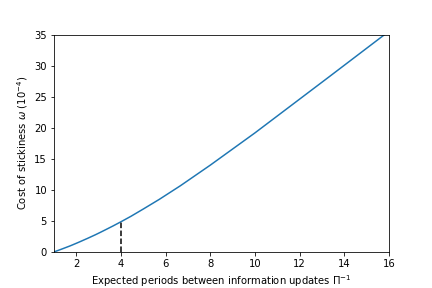
\includegraphics[width=1.5\textwidth]{./Figures/uCostvsPiInv}}
    \end{minipage}
      }
{ 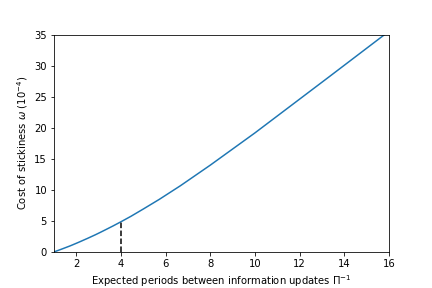
\includegraphics[width=1.0\textwidth]{./Figures/uCostvsPiInv}}
\footnotesize Notes: The figure shows how the utility costs of updating $\omega$ depend on the probability of updating of aggregate information $\Pi$ in the SOE model.
\end{figure}

Now that we have explained how to compute the cost of stickiness numerically, we can test our supposition in equation \eqref{eq:vApproxSticky} that the cost of stickiness might have a roughly inverse linear relationship to $\Pi$.  Figure~\ref{costOfStickiness} plots numerically computed $\omega$ for various values of $\Pi^{-1}$ and is close to linear, as we speculated.



\section{Muth--Lucas--Pischke and \cite{reis:inattentive} Redux} \label{sec:Comparisons}

Now that our calibrations and results have been presented, we are in position to make some quantitative comparisons of our model to two principal alternatives to habit formation (or our model) for explaining excess smoothness in consumption growth.

The longest-standing rival to habit formation as an explanation of consumption sluggishness is what we will call the Muth--Lucas--Pischke (henceforth, MLP) framework.  The idea is not that agents are inattentive, but instead that they have imperfect information on which they (perfectly attentively) perform an optimal signal extraction problem.

\cite{muthOptimal}'s agents could observe only the level of their income, but not the split between its permanent and transitory components.  He derived the optimal (mean-squared-error-minimizing) method for estimating the level of permanent income from the observed signal about the level of actual income.  \cite{lucas:imperfectInfo} applied the same mathematical toolkit to solve a model in which firms are assumed to be unable to distinguish idiosyncratic from aggregate shocks.  \cite{pischkeMicroMacro} combines the ideas of Muth and Lucas and applies the result to the analysis of micro data: His consumers have no ability at all to perceive whether income shocks that hit them are aggregate or idiosyncratic, transitory or permanent.  They see only their income, and do signal extraction on it.

Pischke calibrates his model with micro data in which he calculates that transitory shocks vastly outweigh permanent shocks.\footnote{Pischke's estimates constructed from the {\it Survey of Income and Program Participation} are rather different from the magnitudes of transitory and permanent shocks estimated in the extensive literature---mostly subsequent to Pischke's paper---cited in our calibration section above.}  So, when a shock arrives, consumers always interpret it as being almost entirely transitory and change their consumption by little.  However, macroeconometricians have long known that {\it aggregate} income shocks are close to permanent.  When an aggregate permanent shock comes along, Pischkian consumers spend very little of it, confounding the aggregate permanent shock's effect on their income with the mainly transitory idiosyncratic shocks that account for most of the total variation in their income.  This misperception causes sluggishness in {\it aggregate} consumption dynamics in response to aggregate shocks.  (See below for a more precise formulation of this point).

In its assumption that consumers fail to perceive aggregate shocks immediately and fully, Pischke's model resembles ours.  However, few papers in the literature after \cite{pischkeMicroMacro} have adopted his assumption that households have no idea, when an idiosyncratic income shock occurs, whether it is transitory or permanent.  Especially in the last decade or so, the literature instead has almost always assumed that consumers can perfectly perceive the transitory and permanent components of their income.\footnote{The presumption that permanent idiosyncratic shocks are easily observed is bolstered by the work of \cite{lmp:wagerisk}, who find that most `permanent' changes to individual income income are concentrated in periods when people change jobs or become unemployed or reemployed.  It is simply not plausible to assume that consumers are not aware their income has permanently changed when they take a new job or are fired from an existing one.  Furthermore, there are at least some shocks whose transitory nature is impossible to misperceive; the best example is lottery winnings in Norway, see again \cite{fhnMPC}.  The consumption responses to those shocks resemble the responses measured in the previous literature to shocks that economists presumed (contra Pischke) that consumers knew to be transitory.  If consumers respond to such shocks in ways similar to their responses to unambiguously transitory shocks like lottery winnings, it seems hard to accept Pischke's crucial assumption that consumers treat all income shocks identically because they cannot perceive whether any given shock is transitory or permanent. A further motivation for our choice to assume that consumers perceive their idiosyncratic shocks is that our strategy has been to deviate as little as possible from the well-understood benchmark models in the micro consumption literature, which has become sufficiently widely used that they are the natural base upon which to build.  A final piece of evidence comes from some newly collected data from the Federal Reserve Bank of New York's {\it Survey of Consumer Expectations.}  \cite{kmpIncomeExpectations} report on results from an experiment in which consumers were asked to forecast their future income.  The actual realizations of the same consumer's income were collected in a subsequent wave of the survey.  The principal result is that consumers' mean forecast error was very close to zero.  The authors of the post (entitled ``Understanding Permanent and Temporary Income Shocks'') present the results as a confirmation of modern models' standard assumption that consumers have accurate perceptions of the dynamics of their income.}

Granting our choice to assume that consumers correctly perceive the events that are idiosyncratic to them (job changes, lottery winnings, etc), there is still a potential role for application of the MLP framework:  Instead of assuming sticky expectations, we could instead have assumed that consumers perform a signal extraction exercise on \textit{only} the aggregate component of their income, because they cannot perceive the transitory/permanent split for the (tiny) part of their income change that reflects aggregate macroeconomic developments.

In principle (and more plausibly than under Pischke's assumption of complete ignorance), such confusion could generate excess smoothness.  To see how, note that in the Muth framework, agents update their estimate of permanent income according to an equation of the form:\footnote{$\hat{P}_t$ is used to denote that households do an optimal signal-extraction (as opposed to having sticky expectations resulting in $\perc{P}_t$).}
\begin{eqnarray}
  \label{eq:PischkeP}
  \hat{\PLev}_{t+1} & = & \Pi \mathbf{Y}_{t+1}+(1-\Pi) \hat{\PLev}_{t},
\end{eqnarray}

We can now consider the dynamics of aggregate consumption in response to the arrival of an aggregate shock that (unbeknownst to the consumer) is a permanent shock.  The consumer spends $\Pi$ of the shock in the first period, leaving $(1-\Pi)$ unspent because that reflects the average transitory component of an undifferentiated shock.  However, since the shock really was permanent, income next period does not fall back as the consumer guessed it would on the basis of the mistaken belief that $(1-\Pi)$ of the shock was transitory.  The next-period consumer treats this surprise as a positive shock relative to expected income, and spends the same proportion $\Pi$ out of the perceived new shock.  These dynamics continue indefinitely, but with each successive perceived shock (and therefore each consumption increment) being smaller than the last by the proportion $(1-\Pi)$.  Thus, after a true permanent shock received in period $t$, the full-information prediction of the expected dynamics of future consumption changes would be $\Delta \mathbf{C}_{t+n+1} = (1-\Pi)  \Delta \mathbf{C}_{t+n} + \epsilon_{t+n}$.\footnote{The reciprocal logic would apply in the case of a shock that was known by the econometrician to be perfectly transitory, generating the same serial correlation in predictable consumption growth as in the case of the known-to-be-permanent shock.  The only circumstance under which this serial correlation does {\it not} arise is when the econometrician has exactly the same beliefs as the consumer about the breakdown of the shock between transitory components.  More precisely, it is still the case that the serial correlation coefficient on the predictable component of consumption growth is $(1-\Pi)$.  But that predictable component itself is now zero, and $(1-\Pi)\times0=0$.}

At first blush, this predictability in consumption growth would appear to be a violation of \cite{hallRandomWalk}'s proof that, for consumers who make rational estimates of their permanent income, consumption must be a random walk.  The reconciliation is that what Hall proves is that consumption must be a random walk {\it with respect to the knowledge the consumer has}.  The random walk proposition remains true for consumers whose knowledge base contains only the perceived level of aggregate income.  Our thought experiment was to ask how much predictability would be found by an econometrician {\it who knows more than the consumer} about the level of aggregate permanent income.

The in-principle reconciliation of econometric evidence of predictability/excess smoothness in consumption growth, and the random walk proposition, is therefore that the econometricians who are making their forecasts of aggregate consumption growth use other variables in addition to the lagged history of aggregate income itself (and that those variables have useful predictive power).\footnote{This is logically identical to Pischke's analysis of the case where the macroeconometrician knows that aggregate shocks are permanent, but the microeconomic consumers do not perceive those aggregate permanent shocks.}

We now turn to the question of whether the Muth--Lucas--Pischke story is a good {\it quantitative} explanation of the {\it size} of aggregate excess smoothness.  Appendix~\ref{appendix:Muth} shows that, defining the signal-to-noise ratio $\stnRatio=\sigma_{\Psi}/\sigma_{\Theta}$, Muth's derivations imply that the optimal updating coefficient is:\footnote{As always in a Muth-type model, the consumer is assumed to know $\sigma_{\Psi}$ and $\sigma_{\Theta}$.}    \begin{eqnarray}
\Pi & = & \varphi \sqrt{1+\varphi^{2}/4} - (1/2) \varphi^{2}
  \end{eqnarray}


\providecommand{\PischkePi}{0.83}
\providecommand{\PischkePiCancel}{0.17}
 \providecommand{\fromFile}{false}
 \providecommand{\FileOrNot}{\ifthenelse{\boolean{\fromFile}}}

Plugging our calibrations of $\sigma_{\Psi}$ and $\sigma_{\Theta}$ from section \ref{sec:calibration} into \eqref{eq:muthOptimal}, the model yields a predicted value of \FileOrNot{$1-\Pi \approx \PischkePiCancel$}{$(1-\Pi) \approx \PischkePiCancel $}---very far below the approximately $0.6$ estimate from \cite{hrsHabit} and even farther below our estimate of roughly $0.7$--$0.8$ for U.S.\ data.  This reflects the well-known fact that aggregate income is hard to distinguish from a random walk; if it were perceived to be a perfect random walk with no transitory component at all, the serial correlation in its growth would be zero.\footnote{A further problem with the MLP approach is that it seems implausible to assume that the typical consumer would do a sophisticated Muthian signal extraction problem (really, a special case of the Kalman filter) on a single observed aggregate variable (aggregate income), when they could do much better either by adding a few more variables that are equally easy to observe (interest rates, past consumption growth, etc). If they were really so intently focused on understanding where the aggregate economy is, they could do better yet, and much more easily, just by reading the available news stories reporting on professional forecasters' forecasts.  Discomfort with this somewhat schizophrenic set of assumptions is why in work after \cite{lucas:imperfectInfo}, Lucas moved away from his assumption that microeconomic agents have imperfect information about aggregate data.}

Considerations similar to the foregoing apply, at least to some degree, to the \cite{reis:inattentive} model.  Moreover, that model has a further disadvantage relative to any of the other three stories (habits, MLP, or our model). In Reis's model consumers update their information on a regular schedule; under a plausible calibration of the model, once a year.  One implication of the model is that the change in consumption at the next reset is unpredictable; this implies that aggregate consumption growth would be unpredictable at any horizon beyond, say, the one-year horizon.  But, the habit formation assumption was incorporated into macroeconomic models in large part to explain the fact that consumption growth is forecastable over extended periods---well beyond the one year horizon.  A calibration of the Reis model in which consumers update once a year therefore leaves much of the original puzzle in place.\footnote{A final critique of the Reis model is that, while its simplifying assumptions yield elegant and intuitive results, it is too stylized to be of much practical use in answering many questions beyond its narrow focus on matching aggregate smoothness.  A fiscal policymaker who wants to understand how various alternative policies might play out over the course of the business cycle would have a difficult time extracting plausible answers to questions like ``how much difference would it make to consumption if our fiscal stimulus took the form of extended unemployment benefits versus a temporary income tax cut.''  Our model's much greater fidelity to the microeconomic data means it might be able to provide at least somewhat plausible answers to these kinds of questions.  (Our model is an example of the broader movement in macroeconomics in recent years from the provision of stylized analytical toy models like Reis's to the construction of models that attempt to be taken seriously for a reasonable range of quantitative as well as qualitative predictions.)}


\section{Conclusion} \label{sec:Conclusion}

Using a traditional utility function that does not incorporate habits, the literature on the microfoundations of consumption behavior has made great strides over the past couple of decades in constructing models that are faithful to many of the microeconomic facts about consumption, income dynamics, and the distribution of wealth.  But over roughly the same interval, habit formation has gone from an exotic hypothesis to a standard assumption in the representative agent macroeconomics literature, because habits allow representative agent models to match the measured smoothness in aggregate consumption growth.  This conflict, thrown into sharp focus by the recent meta-analysis of both literatures by \cite{hrsHabit}, is arguably the most important puzzle in the microfoundations of macroeconomic consumption behavior.

Our argument is that this conflict can be resolved by applying insights from the literature on `inattention' that has developed robustly since the early contributions of \cite{simsInattention}, \cite{woodfordImperfect}, \cite{mrSlumps}, and others.  In the presence of such inattention, aggregation of the behavior of microeconomic consumers without habits generates aggregate consumption dynamics that match the `excess smoothness' facts that have induced the representative agent literature to embrace habits.

The sticky expectations assumption is more attractive for modeling consumption than for other areas where it has been more widely applied, because in the consumption context there is a well-defined utility-based metric for calculating the cost of sticky expectations (in contrast, say, with models in which households' inflation expectations are sticky; the cost of misperceiving the inflation rate is unclear).  The cost to consumers of our proposed degree of macroeconomic inattention is quite modest, for reasons that will be familiar to anyone who has worked with both micro and macro data: Idiosyncratic variation is vastly greater than aggregate variation.  This means that the small imperfections in macroeconomic perceptions proposed here have very modest utility consequences.  So long as consumers respond appropriately to their idiosyncratic shocks (which we assume they do), the failure to keep completely up-to-date with aggregate developments simply does not matter much.

While some previous papers have mooted the idea that inattention (or imperfect information) might generate excess smoothness, the modeling question is a quantitative one (`how much excess smoothness can a sensible model explain?').  We argue that the imperfect information models and mechanisms proposed in the prior literature are quantitatively unable simultaneously to match the micro and macro quantitative facts, while our model matches all the main stylized facts from both literatures.

In future work, it would be interesting to enrich the model so that it has plausible implications for how the degree of attention might vary over time or across people, and to connect the model to the available expectations data (for example, measures of consumer sentiment, or measures of uncertainty constructed from news sources, cf \cite{bbdUncertainty}).  Such work might be particularly useful in any attempt to understand how behavioral dynamics change between normal times (in which news coverage of macroeconomic dynamics is not front-page material) and crisis times (in which it {\it is}).

%\pagebreak

\processdelayedfloats

\small
\bibliography{economics,\texname,\texname-Add}
\normalsize
\pagebreak




\appendix

\section*{Appendix}

\section{Representative Agent (RA) Model}\label{sec:RepAgent}

\input\econtexRoot/LaTeX/appendices/RepAgent.tex




\section{Numerical Methods}\label{appendix:Numeric}

\subsection{Solution Methods}\label{appendix:Solution}

\input\econtexRoot/LaTeX/appendices/Solution.tex


\subsection{Simulation Procedures}\label{appendix:Simulation}

\input\econtexRoot/LaTeX/appendices/Simulation.tex


\subsection{Cost of Stickiness Calculation}\label{appendix:uCost}

\input\econtexRoot/LaTeX/appendices/uCost.tex




\section{Additional Calculations}

\subsection{Quadratic Utility Consumption Dynamics}\label{appendix:QuadCDyn}

\input\econtexRoot/LaTeX/appendices/QuadCDyn.tex


%\subsection{Calibration of Aggregate Income Process}\label{appendix:AggCalib}

%\input\econtexRoot/Empirical/US/Results/LaTeX/AggCalibPermTran.tex

%\input Appendix/EYGivenMandL.tex


\subsection{Population Variance of Idiosyncratic Permanent Income}\label{appendix:pss}

\input\econtexRoot/LaTeX/appendices/Blanchard/pVarianceSteadyState.tex

\subsection{Converting Annual to Quarterly Variances for Idiosyncratic Shocks}\label{appendix:Ann2Qtr}

\input\econtexRoot/LaTeX/appendices/Ann2Qtr.tex

\subsection{\cite{muthOptimal} Signal Extraction}\label{appendix:Muth}

\input\econtexRoot/LaTeX/appendices/MuthPre-muthOptimal.texinput
%\input\eq/muthOptimal.tex

\end{document}









